\documentclass[parskip=full, 12pt]{scrartcl}

\usepackage[utf8]{inputenc} 					% Uses UTF8 file encoding for TeX sources
\usepackage[T1]{fontenc}    					% Avoid garbled Unicode text in PDF
\usepackage[german]{babel}  					% German hyphenation, quotes, etc
\usepackage{graphicx}       					% Provides commands for including figures
\usepackage{color}								% Provides color availability
\usepackage{tikz}								% Provides Mind-Map functionality
\usetikzlibrary{mindmap}

% Anmerkung: Dieses Dokument dient anderen Informatikstudenten als inhaltliche Zusammenfassung für den Kurs Softwaretechnik I am Karlsruher Institut für Technologie. Alle Angaben sind ohne Gewähr auf Richtigkeit und Vollständigkeit.

\begin{document}

\begin{titlepage}
\title{Softwaretechnik I}
\author{Björn Holtvogt}
\date{}
\maketitle
\thispagestyle{empty} % Seitenzahl nicht anzeigen		
\begin{tikzpicture}[remember picture, overlay]
\node at (current page.center){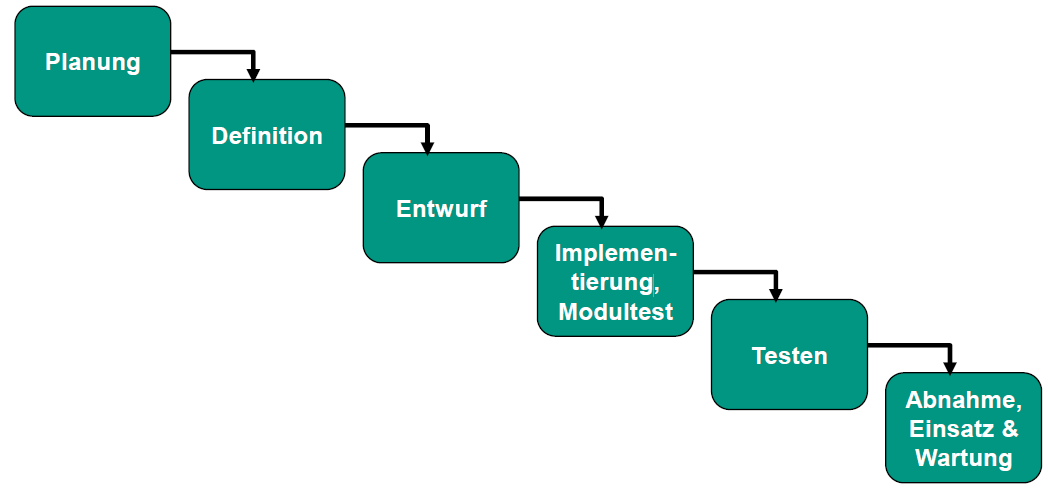
\includegraphics[width=1.1\textwidth]{../images/wasserfallmodell.jpg}};	
\end{tikzpicture}
\begin{center}
Das Wasserfallmodell als einfaches Grundmodell einer softwaretechnischen Planung:
\end{center}
\end{titlepage}
	
% Inhaltsverzeichnis	
% Seitenzahlen im Inhaltsverzeichnis nicht anzeigen
\newpage
\pagestyle{empty}
\tableofcontents	
% Seitenzahlen beginnen wieder bei 1
\newpage
\pagestyle{plain}
\setcounter{page}{1}

% Kapitel
\section{Planungsphase}

Ziel:
\begin{itemize}
\item Beschreibung des Systems in Worten als \textbf{Lastenheft}
\item \textbf{Durchführbarkeitsuntersuchung}
\end{itemize}
	
\subsection{Lastenheft}
	
\begin{itemize}
\item Zielbestimmung
\item Produkteinsatz
\item Funktionale Anforderungen
\begin{itemize}
\item Beschreibt Funktionen, die das System unterstützen muss, unabhängig von der Implementierung
\item Als Aktionen formuliert: \dq Ersterfassung, Änderung und Kunden\dq
\end{itemize}
\item Produktdaten
\item Nichtfunktionale Anforderungen
\begin{itemize}
\item Beschreiben Eigenschaften des Systems: \dq Reagiert innerhalb von zehn Sekunden\dq
\item Als Einschränkung (constraints) oder Zusicherung (assertions) formuliert
\end{itemize}
\item Systemmodelle
\begin{itemize}
\item Szenarien
\item Anwendungsfälle
\end{itemize}
\item Glossar
\begin{itemize}
\item Begriffslexikon zur einheitlichen Kommunikation mit dem Kunden
\end{itemize}
\end{itemize}
		
\subsection{Durchführbarkeitsuntersuchung}
			
\begin{itemize}
\item Fachliche Durchführbarkeit
\begin{itemize}
\item Fachkräfte genügend qualifiziert?
\end{itemize}
\item Alternative Lösungsvorschläge
\begin{itemize}
\item Open-Source als Teilersatz?
\end{itemize}
\item Personelle Durchführbarkeit
\begin{itemize}
\item Genügend qualifizierte Fachkräfte?
\end{itemize}
\item Risiken
\item Ökonomische Durchführbarkeit
\begin{itemize}
\item Projekt wirtschaftlich? (Aufwands- und Terminschätzung, Wirtschaftlichkeitsrechnung)
\end{itemize}
\item Rechtliche Gesichtspunkte
\begin{itemize}
\item Datenschutz
\item Zertifizierung
\end{itemize}
\end{itemize}
\newpage
\section{Definitionsphase}

	Ziel:
	\begin{itemize}
		\item Erstellung eines \textbf{Pflichtenhefts}, mit Hilfe von \textbf{Objekt}- und \textbf{dynamischen Modellen}
	\end{itemize}
		
		\subsection{Pflichtenheft}
			
			\begin{itemize}
				\item  \textbf{Definiert} das zu erstellende System \textbf{vollständig und exakt}
				\begin{itemize}
					\item \underline{Ohne Nachfragen} implementierbar!
					\item Nicht wie, sondern nur \underline{was zu implementieren} ist
				\end{itemize}
				\item Verfeinerung des Lastenhefts
			\end{itemize}
				
		\subsection{Modellarten}
				
			\begin{itemize}
				\item Funktionales Modell (aus dem Lastenheft)
				\begin{itemize}
					\item Szenarien
					\item Anwendungsfalldiagramme
				\end{itemize}
				\item Objektmodell
				\begin{itemize}
					\item Klassendiagramm
					\item Objektdiagramm
				\end{itemize}
				\item Dynamisches Modell
				\begin{itemize}
					\item Sequenzdiagramm
					\item Zustandsdiagramm
					\item Aktivitätsdiagramm
				\end{itemize}
			\end{itemize}
				
		\newpage
		\subsection{Gliederung}
				
			\begin{itemize}
				\item Zielbestimmung 
				\item Produkeinsatz
				\item \textbf{\textit{Produktumgebung}}
				\item Funktionale Anforderungen
				\item Produktdaten
				\item Nichtfunktionale Anforderungen
				\item \textbf{\textit{Globale Testfälle}}
				\item Systemmodelle
				\begin{itemize}
					\item Szenarien
					\item Anwendungsfälle
					\item \textbf{\textit{Objektmodelle}}
					\item \textbf{\textit{Dynamische Modelle}}
					\item \textbf{\textit{Benutzerschnittstelle - Bildschirmskizze, Navigationspfade}}
				\end{itemize}
				\item Glossar
			\end{itemize}
				
		\subsection{Liskov'sches Substitutionsprinzip}
			
			\begin{itemize}
				\item In einem Programm, in dem U eine Unterklasse von K ist, kann \textbf{jedes Exemplar der Klasse K durch ein Exemplar von U ersetzt werden}, wobei das Programm weiterhin \underline{korrekt funktioniert}
			\end{itemize}
				
		\newpage
		\subsection{Folgerungen aus dem Substitutionsprinzip}
			
			\begin{itemize}
				\item Signaturvererbung
				\begin{itemize}
					\item Eine in der Oberklasse definierte und evtl. implementierte Methode überträgt \textbf{nur ihre Signatur} auf die Unterklasse
				\end{itemize}
				\item Implementierungsvererbung
				\begin{itemize}
					\item Eine in der Oberklasse definierte und implementierte Methode überträgt ihre \textbf{Signatur und ihre Implementierung} auf die Unterklasse
									
					$\Rightarrow$ Implementierungsvererbung setzt Signaturvererbung voraus!
				\end{itemize}
				\item Anpassung geerbter Eigenschaften
				\begin{itemize}
					\item Überladen
					\begin{itemize}
						\item Eine geerbte Methode mit gleichem Namen, aber anderer Signatur wird definiert
					\end{itemize}
					\item Überschreiben
					\begin{itemize}
						\item Eine geerbte, \textbf{dynamische} Methode mit gleichem Namen und gleicher Signatur wird \textbf{neu implementiert}
					\end{itemize}
					\item Verdecken
					\begin{itemize}
						\item Eine geerbte, \textbf{statische} Methode mit gleichem Namen und gleicher Signatur wird \textbf{neu implementiert}
					\end{itemize}
				\end{itemize}
				\newpage
				\item Varianz
				\begin{itemize}
					\item Definition
					\begin{itemize}
						\item Parametermodifikation einer überschriebenen Methode
					\end{itemize}
					\item Invarianz
					\begin{itemize}
						\item Der Parametertyp wird nicht modifiziert
					\end{itemize}
					\item Kovarianz
					\begin{itemize}
						\item Der Parametertyp wird spezialisiert
					\end{itemize}
					\item Kontravarianz
					\begin{itemize}
						\item Der Parametertyp wird allgemeiner
					\end{itemize}
				\end{itemize}
			\end{itemize}
				
			\subsubsection{Varianzen gemäß dem Substitutionsprinzip und in Java}
			
				\begin{center}
					\resizebox{\textwidth}{!}{
					\begin{tabular}{l|c|c|c|c|c|c}
						                              & \multicolumn{3}{c|}{\textbf{Eingabeparameter}} & \multicolumn{3}{c}{\textbf{Ausgabeparameter} } \\
						\hline
						                              & Invarianz                                      & Kovarianz & Kontravarianz & Invarianz & Kovarianz & Kontravarianz \\
						\hline
						\textbf{Substitutionsprinzip} & $\surd$                                        &           & $\surd$       & $\surd$   & $\surd$   & \\
						\hline
						\textbf{Java}                 & $\surd$                                        &           &               & $\surd$   & $\surd$   & \\
					\end{tabular}}
				\end{center}
		
		\subsection{Kapselungsprinzip}
				
			\begin{itemize}
				\item Der \textbf{Zustand} ist zwar nach außen sichtbar, er wird aber \textbf{im Inneren des Objektes verwaltet} (und also nur kontrolliert geändert)
			\end{itemize}
				
		\subsection{Geheimnisprinzip}
			
			\begin{itemize}
				\item Jedes Modul verbirgt eine \textbf{wichtige Entwurfsentscheidung} hinter einer \textbf{wohldefinierten Schnittstelle} die sich bei einer Änderung der Entscheidung \underline{nicht} mit ändert
				\begin{itemize}
					\item \underline{Verborgenes und Unbenutztes} kann ohne Risiko geändert werden
				\end{itemize}
			\end{itemize}
				
		\subsection{Beispiele für Verbergung}
				
			\begin{itemize}
				\item \textbf{Datenstrukturen} (Wahl, Größe und Implementierung und Operationen an diesen)
				\item \textbf{Maschinennahe Details} (Gerätetreiber, Ein- und Ausgabe)
				\item \textbf{Betriebssystemnahe Details} (Ein- und Ausgabeschnittstellen, Dateiformate, Netzwerkprotokolle)
				\item \textbf{Grundsoftware} (Datenbanken, Oberflächenbibliotheken)
				\item \textbf{Benutzungsschnittstellen} (Kommandoschnittstelle, graphische Oberfläche, Gesten-gesteuerte Oberfläche, Web, Sprachsteuerung, Kombinationen davon,..)
				\item \textbf{\underline{Sprache}} (Text von Dialogen, Beschriftungen)
				\item \textbf{Reihenfolge der Verarbeitung}
			\end{itemize}
\newpage
\section{Entwurfsphase}
	
Ziel:
\begin{itemize}
\item Aus \underline{gegebenen Anforderungen} an einem Softwareprodukt wird eine \newline \underline{softwaretechnische Lösung}, die \textbf{Softwarearchitektur}, entwickelt
\end{itemize}
	
\subsection{Softwarearchitektur}
		
\begin{itemize}
\item Gliederung eines Softwaresystems in \textbf{Komponenten} (Module, Klassen) und \textbf{Subsysteme} (Pakete, Bibliotheken)
\item \textbf{Spezifikationen} der Komponenten und Subsystemen
\begin{itemize}
\item Aufstellung der \textbf{Benutztrelation}
\end{itemize}
\end{itemize}
	
\subsection{Entwurfsmethoden}
		
\begin{itemize}
\item \textbf{Modularer Entwurf}
\item \textbf{Objekt-orientierter-Entwurf}
\begin{itemize}
\item Erweiterung um Vererbung, Polymorphie und Datenmodellierung
\end{itemize}
\end{itemize}

\subsection{Modul}

\begin{itemize}
	\item Ist eine \textbf{Menge von Programmelementen} (Typen, Klassen, Konstanten, Variablen, Datenstrukturen, Prozeduren, Funktionen,..), die nach dem \textbf{Geheimnisprinzip} gemeinsam entworfen und geändert werden
\end{itemize}

\subsection{Anforderungen an ein Modul}

\begin{itemize}
\item Module sollen unabhängig voneinander bearbeitet und benutzt werden können
\begin{itemize}
\item \underline{Ohne Kenntnis} der späteren Nutzung entworfen, implementiert und getestet
\end{itemize}
\end{itemize}
	
\newpage
\subsection{Architekturstile}
		
\begin{itemize}
\item Schichtenarchitektur
\item Klient/Dienstgeber (Client/Server)
\item Partnernetze (Peer-To-Peer)
\item Datenablage (Repository)
\item Modell-Präsentation-Steuerung (Model-View-Controller)
\item Fließband (Pipeline)
\item Rahmenarchitektur (Framework)
\item Dienstorientierte Architektur (Service oriented architecture)
\end{itemize}
		
\subsubsection{Schichtenarchitektur}
			
\begin{itemize}
\item Gliederung einer Softwarearchitektur mit \textbf{hierarchischen Schichten}
\begin{itemize}
\item Eine Schicht \underline{nutzt die darunter liegenden Schichten}  und diese \newline stellen ihre Dienste \underline{den darüber liegenden Schichten zur Verfügung}
\end{itemize}
\item Transparent:
\end{itemize}		
				
\begin{center}
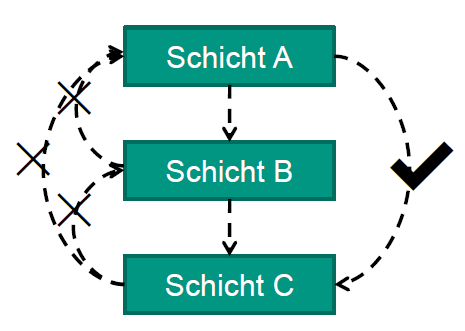
\includegraphics[width=0.5\textwidth]{../images/transparenteSchichtenarchitektur.png}
\end{center}
		
\newpage
\begin{itemize}	
\item Intransparent:	
\end{itemize}		
		
\begin{center}
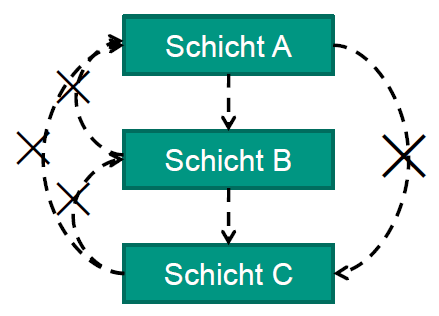
\includegraphics[width=0.5\textwidth]{../images/intransparenteSchichtenarchitektur.png}
\end{center}

\begin{itemize}	
\item 3-\textbf{stufige} Architektur
\begin{itemize}
\item 3-Schichten Architektur mit Schichten auf \underline{unterschiedlichen Rechnern}
\end{itemize}
\item 3-\textbf{Schichten} Architektur
\begin{itemize}
\item Benutzerschnittstelle, Anwendungskern und Datenbanksystem
\end{itemize}
\end{itemize}		
Oft wird die Schichtenarchitektur mit dem Entwurfsmuster \textbf{Fassade} verwendet.
\begin{itemize}
\item Leitet an die eigentlichen Elemente in der Schicht weiter
\end{itemize}
				
\begin{center}
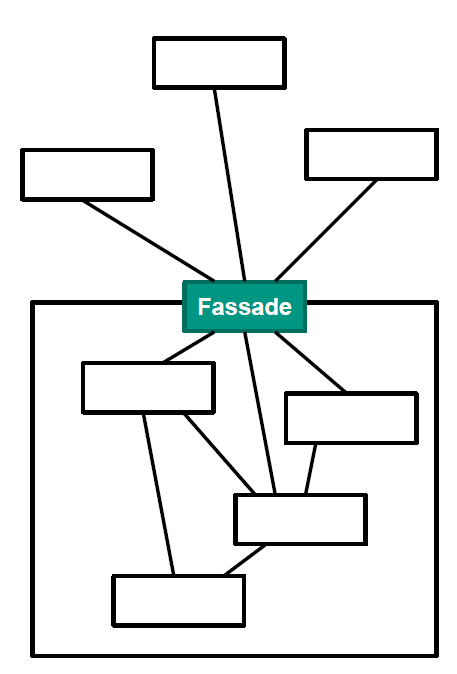
\includegraphics[width=0.3\textwidth]{../images/fassadeSchichtenarchitektur.png}
\end{center}
				
\subsubsection{Klient/Dienstgeber}
				
\begin{itemize}
\item Ein- oder mehrere \textbf{Dienstgeber bieten Dienste für andere Subsysteme} (Klienten) an
\begin{center}
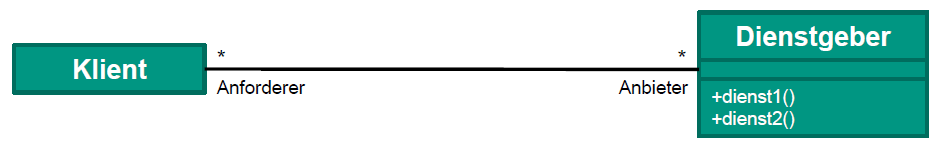
\includegraphics[width=0.9\textwidth]{../images/klientDienstgeber.png}
\end{center}
\item Oft bei \textbf{Datenbankservern} verwendet
\begin{itemize}
\item \underline{Front-End:} Benutzeroberfläche für den Benutzer (Klient)
\item \underline{Back-End}: Datenbankzugriff und Manipulation (Dienstgeber)
\end{itemize}
\item \textbf{Klientenfunktionen}
\begin{itemize}
\item Eingaben des Benutzer entgegennehmen und vor verarbeiten
\end{itemize}
\item \textbf{Dienstgeberfunktionen}
\begin{itemize}
\item Datenverwaltung, -integrität und -konsistenz
\item Sicherheit
\end{itemize}		
\item Beispiel: TCP/IP, DNS (Netzwerkebene)		
\end{itemize}	
	
\subsubsection{Partnernetze}
			
\begin{itemize}
\item \textbf{Verallgemeinerung} von Klient/Dienstgeber
\item Alle Subsysteme sind \textbf{gleichberechtigt}
\begin{center}
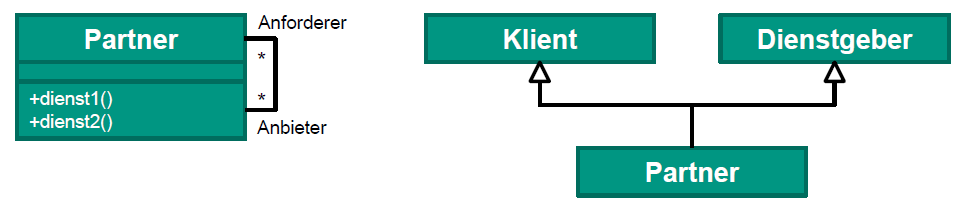
\includegraphics[width=0.9\textwidth]{../images/partnernetze.png}
\end{center}
\end{itemize}
			
\subsubsection{Datenablage}
			
\begin{itemize}
\item Subsysteme \textbf{verändern Daten} von einer zentralen Datenstruktur (Datenablage)
\begin{itemize}
\item Sind \textbf{lose gekoppelt} und interagieren nur über die Datenablage
\end{itemize}
\item Realisierung: \textbf{Lokaler- oder Fernzugriff}
\begin{center}
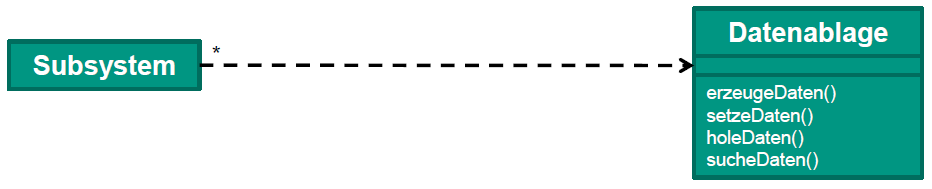
\includegraphics[width=0.9\textwidth]{../images/datenablage.png}
\end{center}
\item Beispiele: Subversion, GIT
\end{itemize}
	
\subsubsection{Modell-Präsentation-Steuerung}
			
\begin{center}
\begin{tabular}{c|c}
\textbf{Problem} & \textbf{Lösung} \\
\hline
System mit \underline{hoher Kopplung} & MVC mit \textbf{Trennung} von Daten und Darstellung
\end{tabular}
\end{center}
			
\begin{itemize}
\item \textbf{Modell:}
\begin{itemize}
\item Verantwortlich für \underline{anwendungsspezifische Daten}
\end{itemize}
\item \textbf{Präsentation:}
\begin{itemize}
\item Verantwortlich für die \underline{Darstellung} der Objekte der Anwendung
\end{itemize}
\item \textbf{Steuerung:}
\begin{itemize}
\item Verantwortlich für \underline{Benutzerinteraktion}
\item \underline{Aktualisiert} Modell
\item Weiterleitung der \underline{Änderung von Modelldaten} an Präsentation
\end{itemize}
$\Rightarrow$ Entwurfsmuster: \textbf{Beobachter}!
\end{itemize}
	
\begin{center}
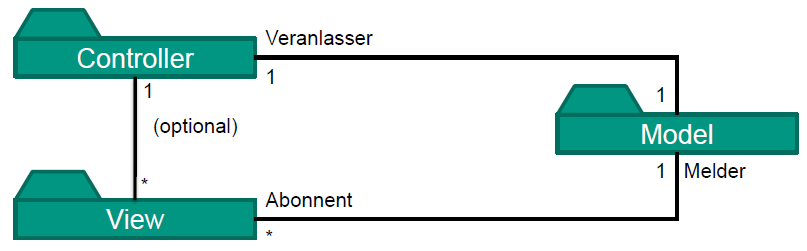
\includegraphics[width=0.9\textwidth]{../images/mvc.png}
\end{center}
	
\subsubsection{Fließband}
			
\begin{itemize}
\item Jede/r Stufe/Filter ist ein \textbf{eigenständiger- und ablaufender Prozess/Faden}
\item Jede Stufe \textbf{verarbeitet vorherige Daten} und sendet sie an die nächste Stufe
\end{itemize}
	
\begin{center}
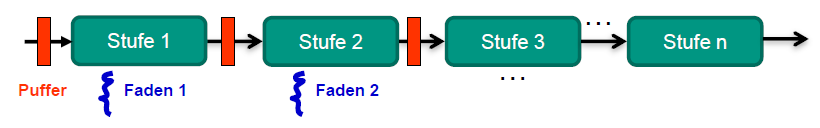
\includegraphics[width=0.8\textwidth]{../images/fliessband.png}
Bei Parallelrechnern echt parallel ausführbar!
\end{center}
	
\begin{itemize}
\item Beispiel: Unix-Shell
\item \textbf{Anwendung:}
\begin{itemize}
\item Datenströme (Videobearbeitung, Übersetzer, Stapelverarbeitung)
$\Rightarrow$ Für \textbf{gute Leistung}: Einzelne Stufen etwa \underline{gleich schnell} ausführbar auf Parallelrechnern
\end{itemize}
\end{itemize}
	
\subsubsection{Rahmenarchitektur}
			
\begin{itemize}
\item Bietet \textbf{fast vollständiges Programm}, dass durch \textbf{Lücken/Erweiterungen} erweitert werden kann
\item \textbf{Klassenabstrahierung} und \textbf{Methodenüberschreibung} vorgesehen
\begin{itemize}
\item Rahmenprogramm führt Erweiterungen (\textbf{Plug-Ins}) richtig aus
\end{itemize}
\end{itemize}
			
\underline{Herkömmlich:}
\begin{itemize}
\item Hersteller liefert Bibliotheken
\item Benutzer schreibt Hauptprogrammlogik
\end{itemize}
			
\begin{center}

\includegraphics[width=0.8\textwidth]{../images/rahmenarchitekturHerkoemmlich.png}
\end{center}
				
\underline{Mit Rahmenarchitektur:}
\begin{itemize}
\item \textbf{Hollywood-Prinzip}: Don't call us, we call you!
\item Hauptprogramm vorhanden, Erweiterungen vom Benutzer werden aufgerufen
\end{itemize}
	
\begin{center}
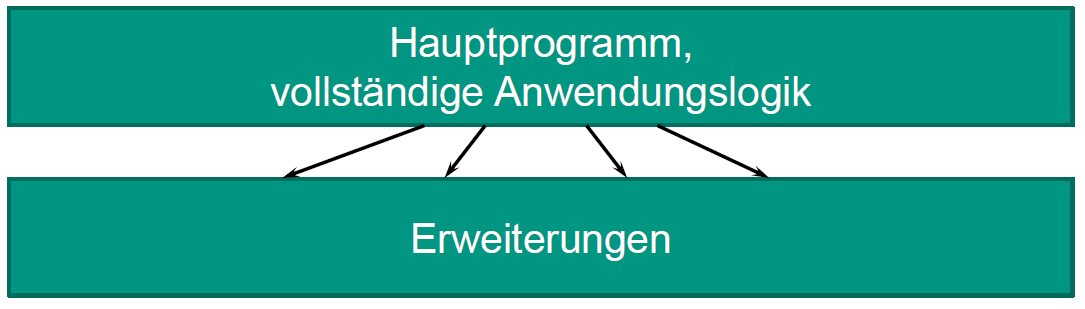
\includegraphics[width=0.8\textwidth]{../images/rahmenarchitektur.png}
\end{center}
	
\newpage
\underline{Beispiel:}
				
\begin{center}
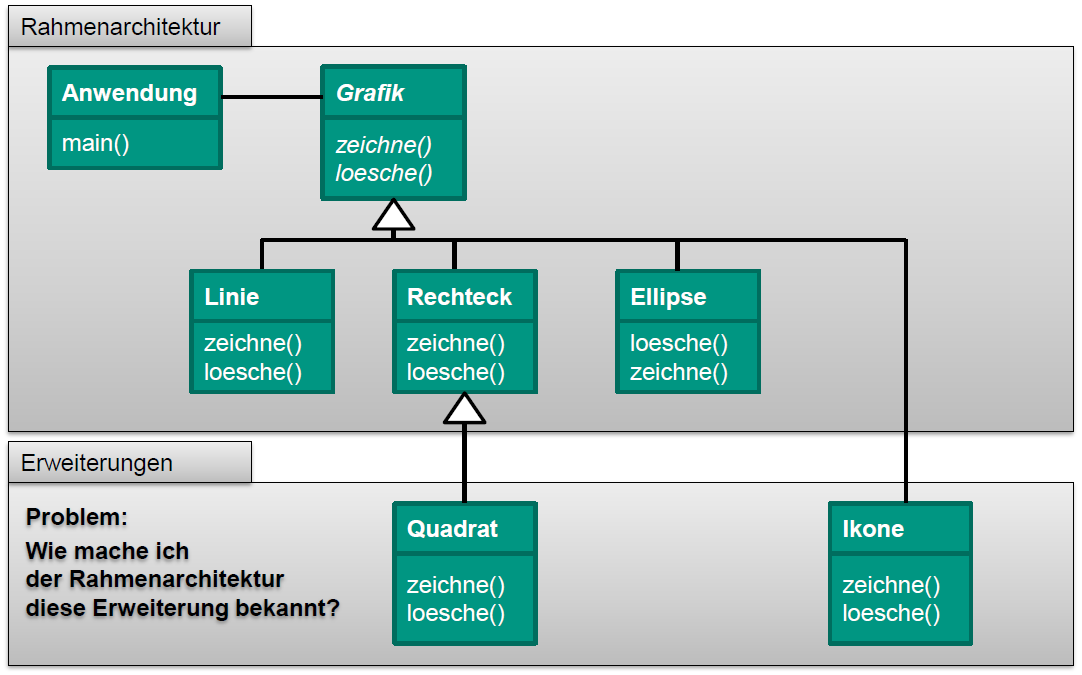
\includegraphics[width=0.9\textwidth]{../images/rahmenarchitekturBeispiel.png}
\end{center}

\begin{itemize}
\item \textbf{Anwendung:}
\begin{itemize}
\item \underline{Grundversion} der Anwendung schon funktionsfähig
\item Erweiterung \underline{konsistent}
\item \textbf{Entwurfsmuster:} Strategie, Fabrikmethode, Abstrakte Fabrik und Schablonenmethode
\end{itemize}
\end{itemize}
	
\subsubsection{Dienstorientierte Architekturen}
		
\begin{itemize}
\item Anwendungen bestehen aus \textbf{unabhängigen Diensten}
\begin{itemize}
\item Abstraktes Konzept
\end{itemize}
\item Dienste als \textbf{zentrale Elemente} eines Unternehmens
\begin{itemize}
\item Bereitstellen gekapselter Funktionalität an andere Dienste/Anwendungen
\begin{itemize}
\item \textbf{Gemeinsame Schnittstelle} für standardisierte(r) Austausch/Kommunikation
\end{itemize}
\end{itemize}
\item \underline{Merkmale/Ziele:}
\begin{itemize}
\item \textbf{Lose Kopplung}
\begin{itemize}
\item \underline{Einfaches Ersetzen} eines Dienstes zur Laufzeit
\item \underline{Dynamisches Binden} durch Dienstverzeichnis
\end{itemize}
\item \textbf{Unterstützung von Geschäftsprozessen}
\begin{itemize}
\item Dienste kapseln geschäftsrelevante Funktionalität
\end{itemize}
\item \textbf{Verwendung von offenen Standards!}
\begin{itemize}
\item \underline{Programmiersprachen}- und \underline{plattformunabhängige} Bereitstellung von Diensten
\end{itemize}
\end{itemize}
\end{itemize}
	
\begin{center}
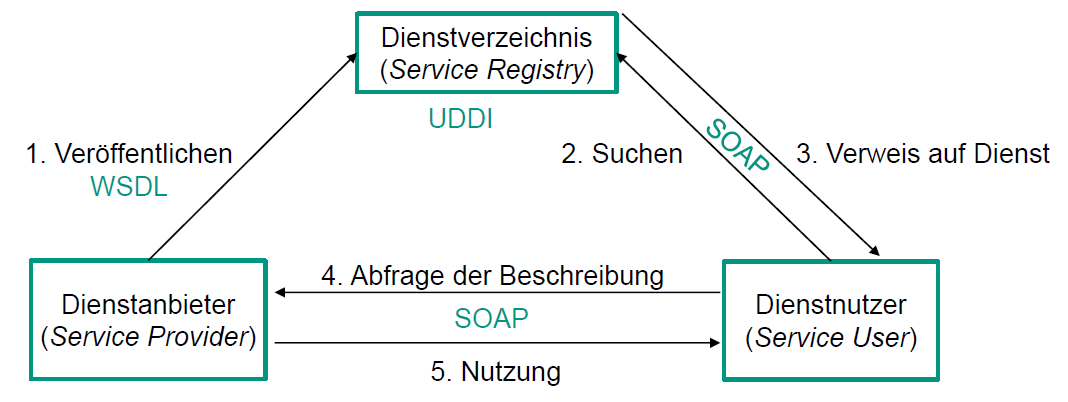
\includegraphics[width=0.9\textwidth]{../images/dienstorientierteArchitektur.png}				
$\Rightarrow$ \textbf{Dienstmodell} als Kern der Dienstorientierten Architektur
\end{center}

\subsection{Entwurfsmuster}
					
\resizebox{\textwidth}{!}{
\begin{tikzpicture}[mindmap, grow cyclic, text centered, every node/.style=concept, concept color=blue!60, level 1/.append style={text width=2.5cm, level distance=5.5cm,sibling angle=72}, level 2/.append style={text width=1.75cm, level distance=3.25cm,sibling angle=40}] 
				
\node{Entwurfsmuster}
child {node {Entkopplungs\\muster}
child {node {Adapter}}
child {node {Beobachter}}
child {node {Brücke}}
child {node {Iterator}}
child {node {Stell\\vertreter}}
child {node {Vermittler}}
}
child { node {Steuerungs\\muster}
child {node {Befehl}}
child {node {Master/\\Worker}}
}
child { node {Zustands\\handhabungs\\muster}
child {node {Einzel\\stück}}
child {node {Prototyp}}
child {node {Memento}}
child {node {Fliegen\\gewicht}}
child {node {Zustand}}
}
child { node {Varianten\\muster}
child {node {Abstrakte\\Fabrik}}
child {node {Dekorierer}}
child {node {Strategie}}
child {node {Kompo\\situm}}
child {node {Besucher}}
child {node {Fabrik\\methode}}
child {node {Schablonen\\methode}}
}
child { node {Bequemlich\\keitsmuster}
child {node {Null-Objekt}}
child {node {Fassade}}
child {node {Bequem\\lichkeits\\methode}}
child {node {Bequem\\lichkeits\\klasse}}
};
\end{tikzpicture}}
	
\newpage
\begin{itemize}
\item \textbf{Entkopplungsmuster:}
\begin{itemize}
\item Teilt System in \textbf{unabhängige Einzelsysteme}
\begin{itemize}
\item \underline{Vorteil}: Durch lokale Änderungen \textbf{verbesser}-, \textbf{anpass}- und \textbf{erweiterbar} \underline{ohne} ganzes System zu modifizieren
\end{itemize}
\end{itemize}
\item \textbf{Variantenmuster:}
\begin{itemize}
\item \textbf{Herausziehen von Gemeinsamkeiten} und platzieren an \underline{einer} Stelle
\begin{itemize}
\item \underline{Vorteil}: \textbf{Keine Codewiederholung}
\end{itemize}
\end{itemize}
\item \textbf{Zustandshandhabungsmuster:}
\begin{itemize}
\item \textbf{Bearbeitung des Zustands} von Objekten unabhängig vom Zweck
\end{itemize}
\item \textbf{Steuerungsmuster:}
\begin{itemize}
\item \textbf{Kontrollflusssteuerung} (Aufruf der richtigen Methode zur richtigen Zeit)
\end{itemize}
\item \textbf{Bequemlichkeitsmuster:}
\begin{itemize}
\item \underline{Sparen} von \textbf{Schreib- und Denkarbeit}
\end{itemize}
\end{itemize}

\newpage
\subsubsection{Entkopplungsmuster}
				
\begin{itemize}
\item \textbf{Adapter} (Wrapper)
\begin{itemize}
\item \textbf{Passt die Schnittstelle einer Klasse an} eine andere, \textbf{vom Klienten erwartete Schnittstelle} an
\end{itemize}
\begin{center}
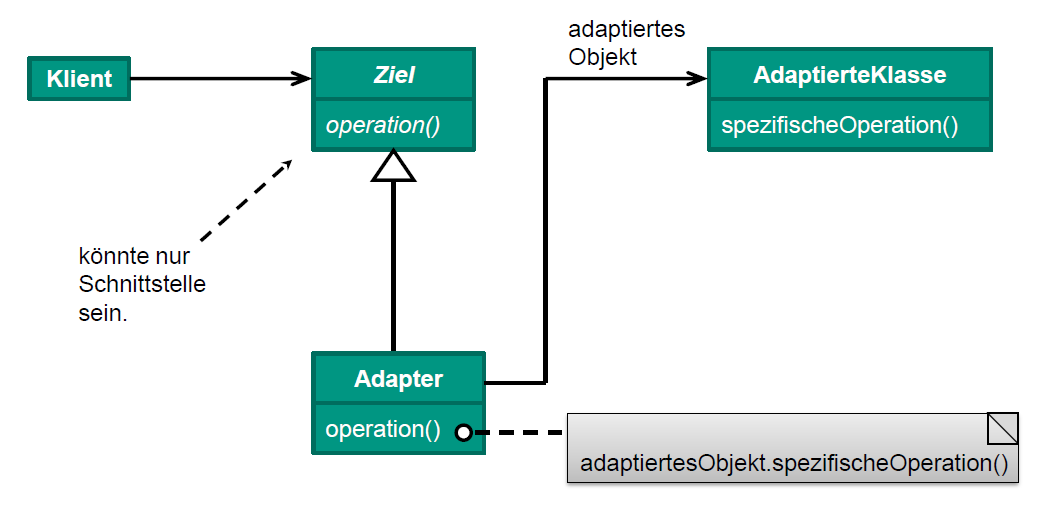
\includegraphics[width=0.9\textwidth]{../images/adapter.png}
\end{center}
\item \textbf{Beobachter} (Observer)
\begin{itemize}
\item \textbf{1:n Abhängigkeit} zwischen Objekten, so dass die \textbf{Änderung eines Zustandes} eines Objektes dazu führt, dass alle abhängigen Objekte \textbf{benachrichtigt und aktualisiert} werden
\end{itemize}
\begin{center}
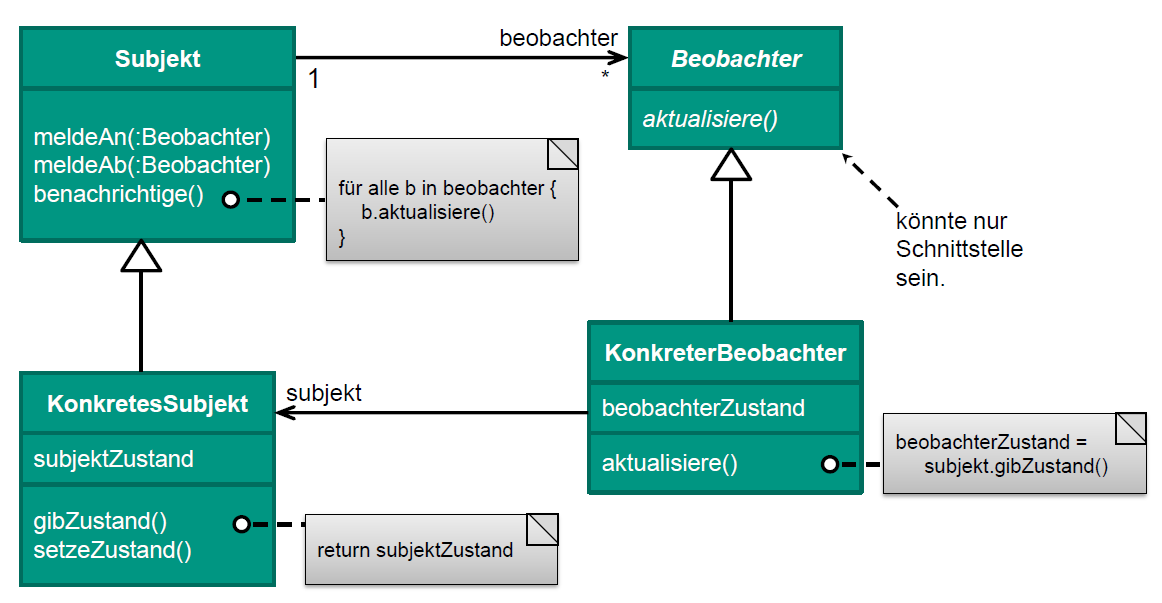
\includegraphics[width=0.9\textwidth]{../images/beobachter.png}
\end{center}
\item \textbf{Brücke} (Bridge)
\begin{itemize}
\item \textbf{Entkoppelt eine Abstraktion von ihrer Implementierung}, so dass beide \textbf{unabhängig voneinander variiert} werden können
\end{itemize}
\begin{center}
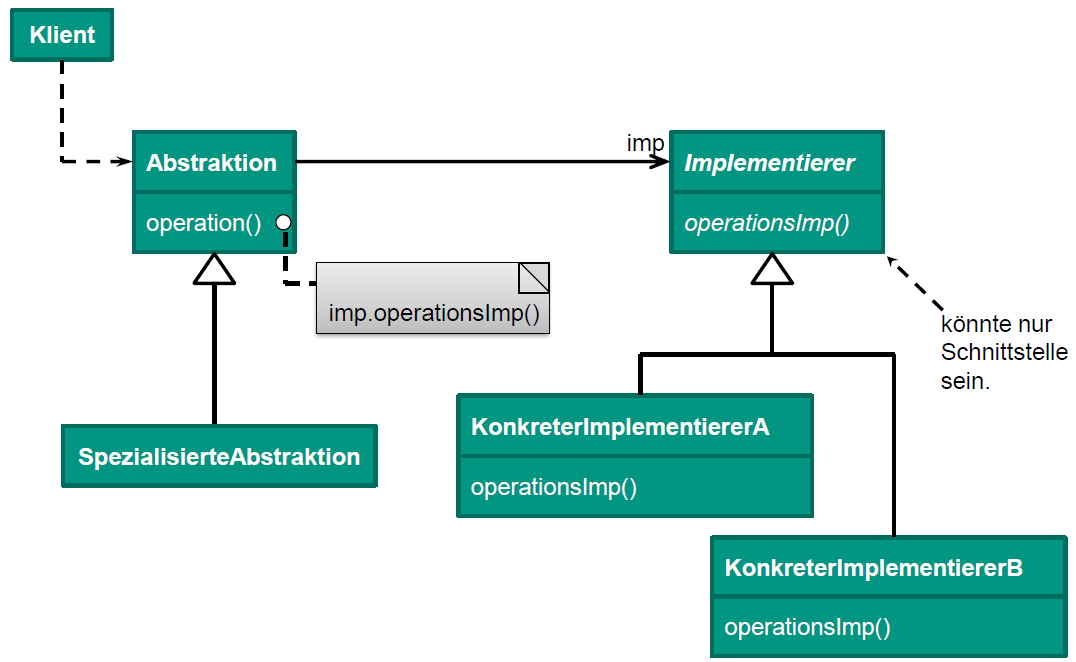
\includegraphics[width=0.8\textwidth]{../images/bruecke.png}
\end{center}
\item \textbf{Iterator}
\begin{itemize}
\item Ermöglicht \textbf{sequentiellen Zugriff} auf die Elemente eines zusammengesetzten Objektes, \textbf{ohne seine zugrundeliegende Repräsentation offenzulegen}
\end{itemize}
\begin{center}
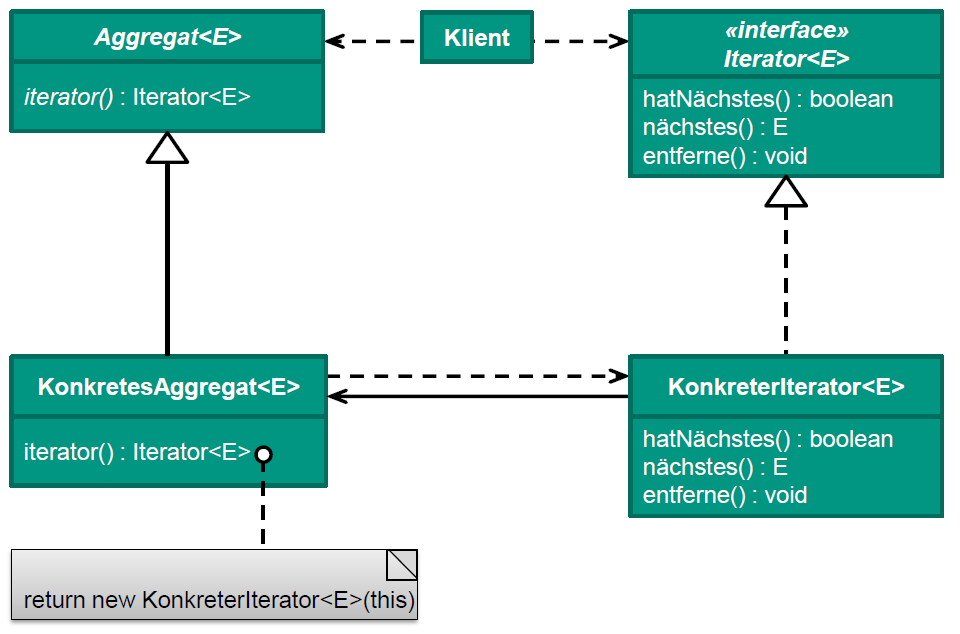
\includegraphics[width=0.7\textwidth]{../images/iterator.png}
\end{center}
\item \textbf{Stellvertreter} (Proxy)
\begin{itemize}
\item \textbf{Kontrolliert den Zugriff auf ein Objekt}, mit Hilfe eines \textbf{vorgelagerten Stellverteterobjekts}
\end{itemize}
\begin{center}
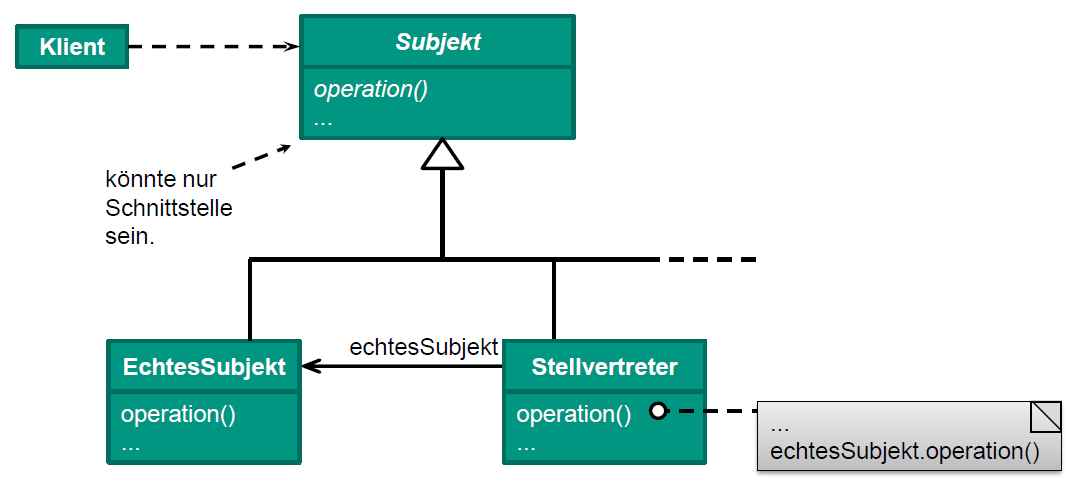
\includegraphics[width=0.9\textwidth]{../images/stellvertreter.png}
\end{center}
\item \textbf{Vermittler} (Mediator)
\begin{itemize}
\item Definiert ein Objekt, dass das \textbf{Zusammenspiel einer Menge von Objekten} in sich kapselt
$\Rightarrow$ \textbf{Zentralisieren}!
\end{itemize}
\begin{center}
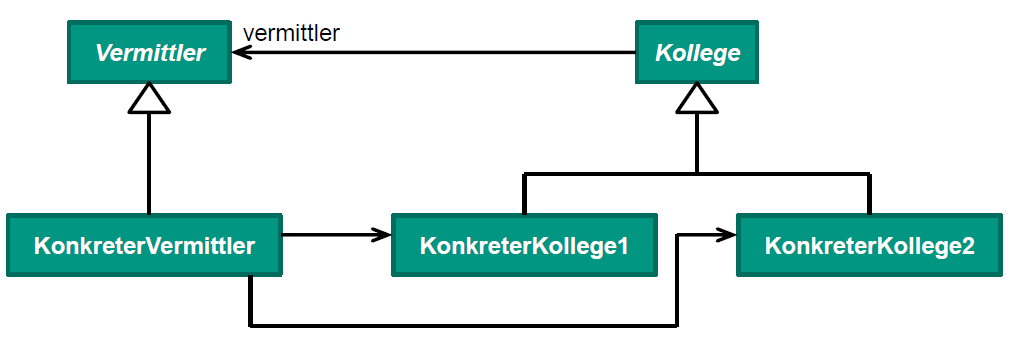
\includegraphics[width=0.9\textwidth]{../images/vermittler.png}
\end{center}
\end{itemize}
			
\newpage
\subsubsection{Variantenmuster}
		
\begin{itemize}
\item \textbf{Abstrakte Fabrik}
\begin{itemize}
\item Bietet eine Schnittstelle zum \textbf{Erzeugen von Familien} \underline{verwandter} oder \newline \underline{voneinander abhängigen Objekte}, ohne ihre konkreten Klassen zu benennen
\end{itemize}
\begin{center}
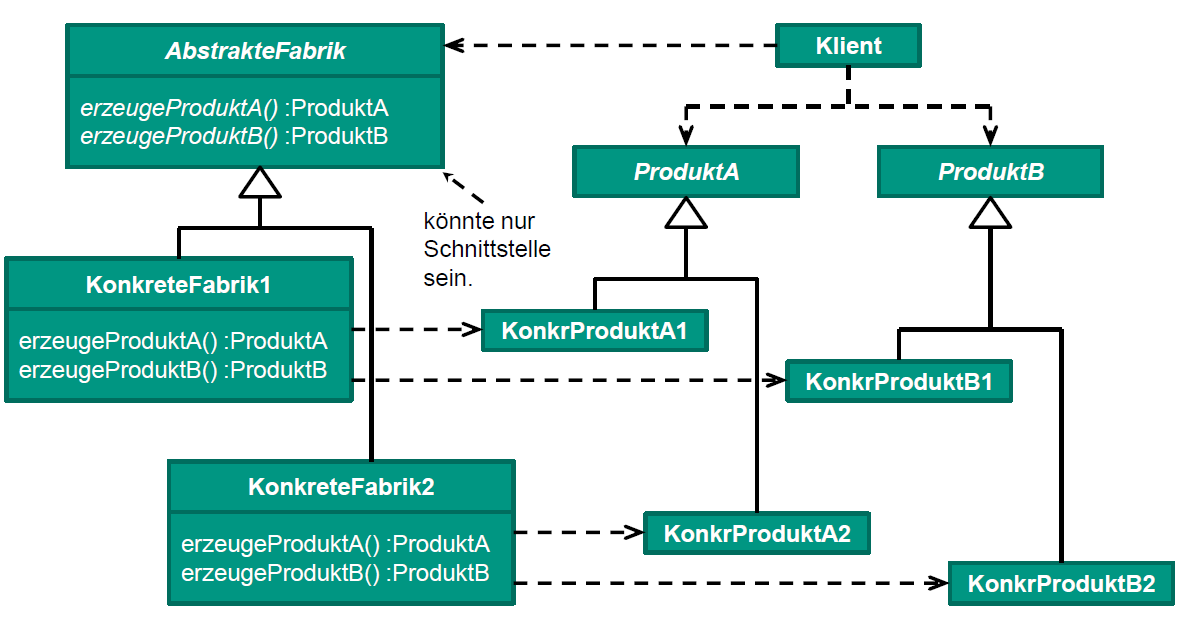
\includegraphics[width=0.8\textwidth]{../images/abstrakteFabrik.png}
\end{center}
\item \textbf{Besucher} (Visitor)
\begin{itemize}
\item \textbf{Kapselt} eine auf den Elementen einer Objektstruktur \textbf{auszuführenden Operation} als ein Objekt
\end{itemize}
\begin{center}
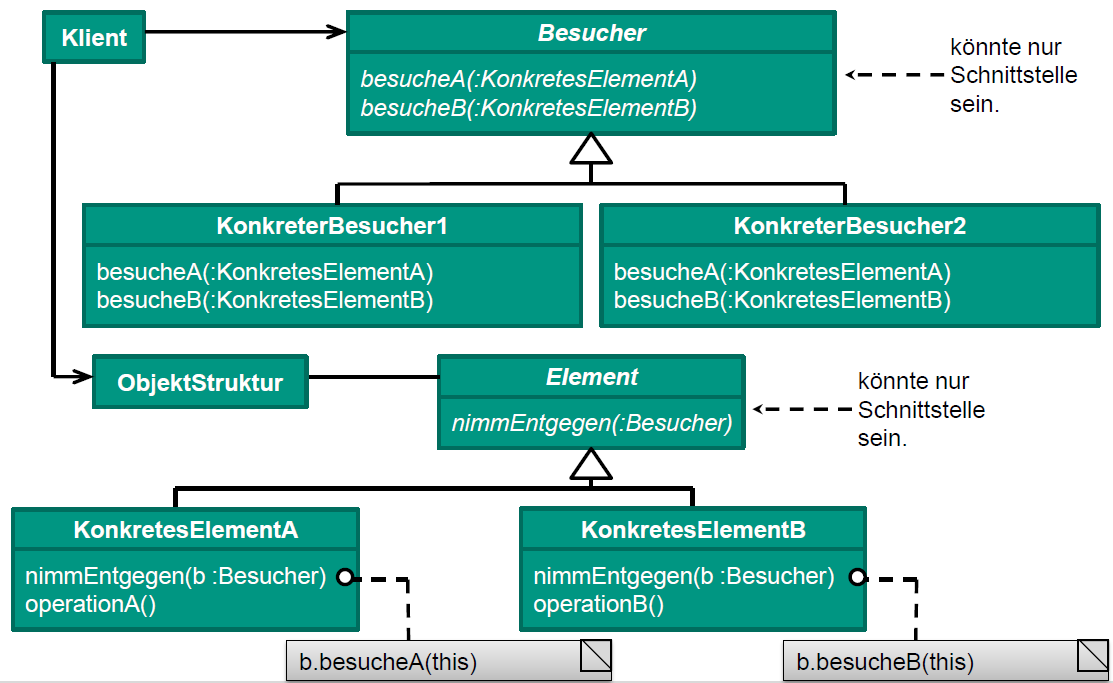
\includegraphics[width=0.8\textwidth]{../images/besucher.png}
\end{center}
\item \textbf{Schablonenmethode} (Template Method)
\begin{itemize}
\item Definiert \textbf{in einer Methode das Skelett eines Algorithmus} und überlässt einzelne Schritte den Unterklassen
\end{itemize}
\begin{center}
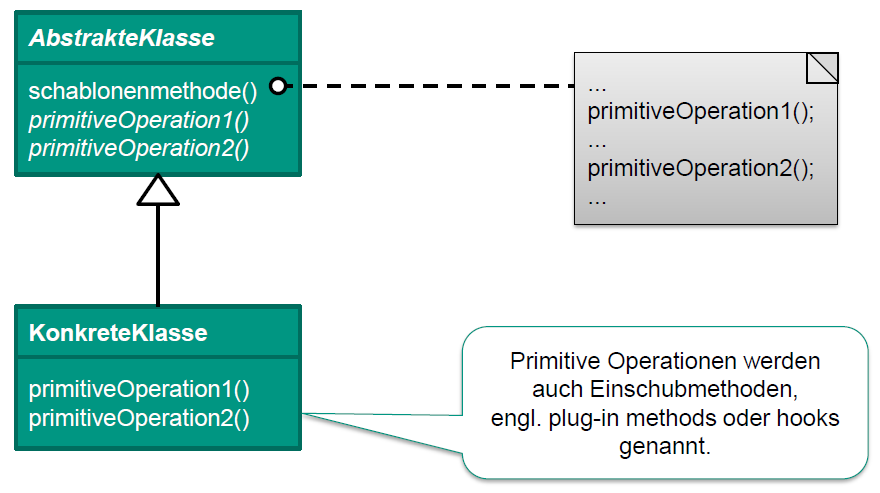
\includegraphics[width=0.9\textwidth]{../images/schablonenmethode.png}
\end{center}
\item \textbf{Fabrikmethode} (Factory Method)
\begin{itemize}
\item Definiert eine \textbf{Klassenschnittstelle mit Operationen zum Erzeugen} eines Objekts, aber \textbf{lässt Unterklassen entscheiden, von welcher Klasse} das zu erzeugende Objekt ist
\end{itemize}
\begin{center}
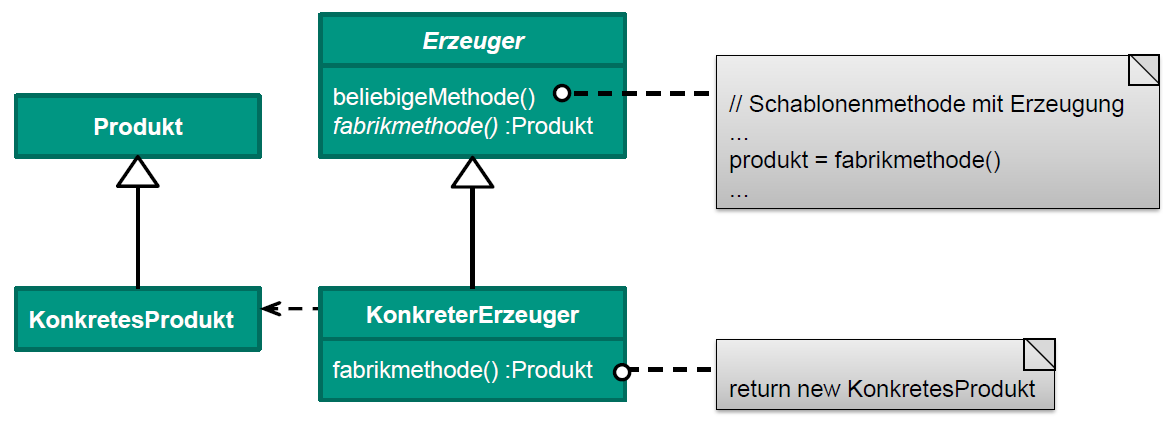
\includegraphics[width=0.9\textwidth]{../images/fabrikmethode.png}
\end{center}
\newpage
\item \textbf{Kompositum}
\begin{itemize}
\item Fügt Objekte zu \textbf{Baumstrukturen} zusammen, um \textbf{Bestandshierarchien} zu repräsentieren. Ermöglicht, das \textbf{Klienten, einzelne Objekte und Aggregate einheitlich} behandelt werden
\end{itemize}
\begin{center}
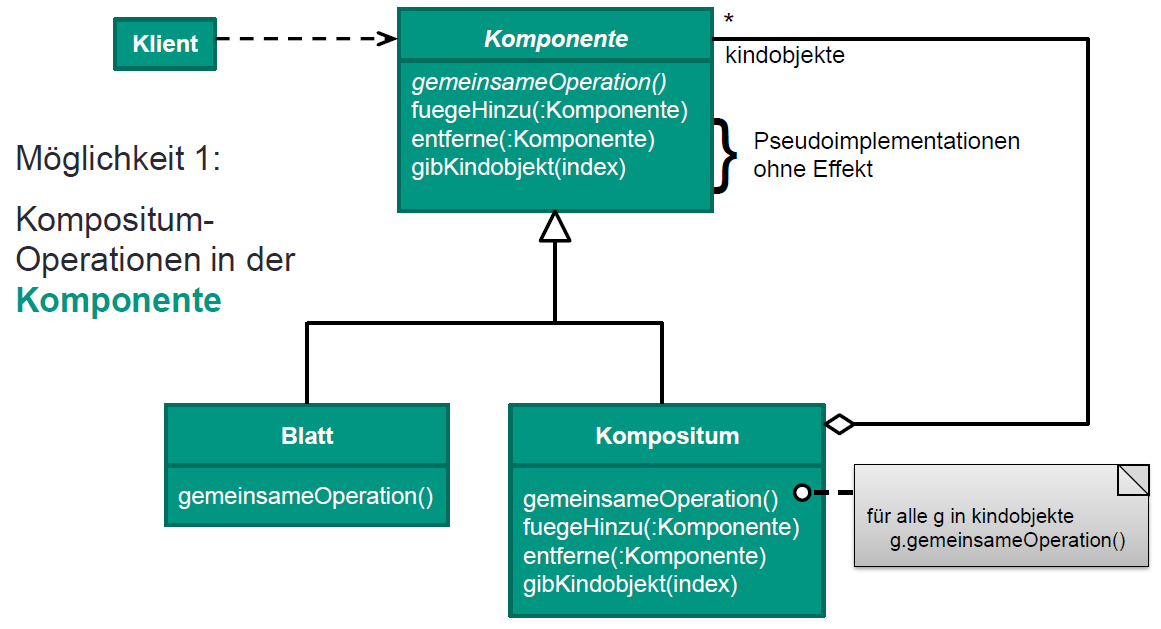
\includegraphics[width=0.9\textwidth]{../images/kompositum.png}
\end{center}
\item \textbf{Strategie} (Stichwort: Switch-less programming)
\begin{itemize}
\item Definiert eine \textbf{Familie von Algorithmen}, \textbf{kapselt} sie und macht sie \textbf{austauschbar}
\end{itemize}
\begin{center}
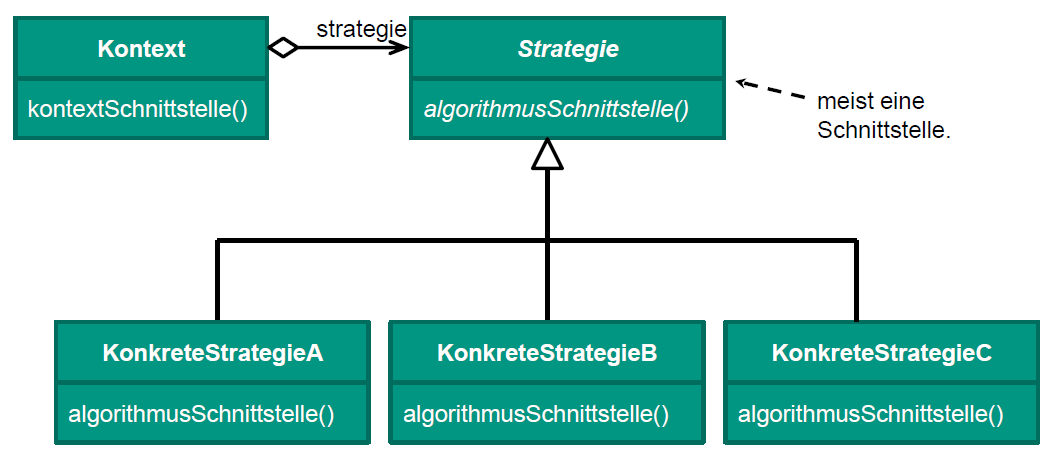
\includegraphics[width=0.9\textwidth]{../images/strategie.png}
\end{center}
\newpage
\item \textbf{Dekorierer}
\begin{itemize}
\item Fügt \textbf{dynamisch zur Laufzeit neue Funktionalitäten} zu einem Objekt hinzu
\end{itemize}
\begin{center}
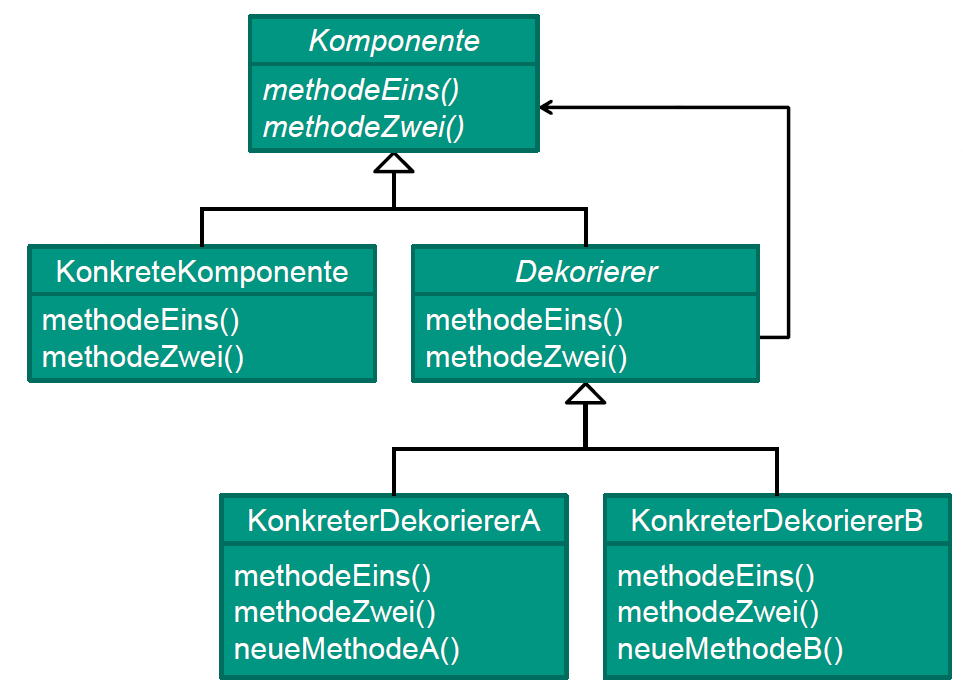
\includegraphics[width=0.6\textwidth]{../images/dekorierer.png}
\end{center}
\end{itemize}
			
\subsubsection{Zustandshandhabungsmuster}
			
\begin{itemize}
\item \textbf{Einzelstück} (Singleton)
\begin{itemize}
\item Zusicherung, dass eine Klasse \textbf{genau ein Exemplar} besitzt mit \textbf{globalen Zugriffspunkt}
\end{itemize}
\begin{center}
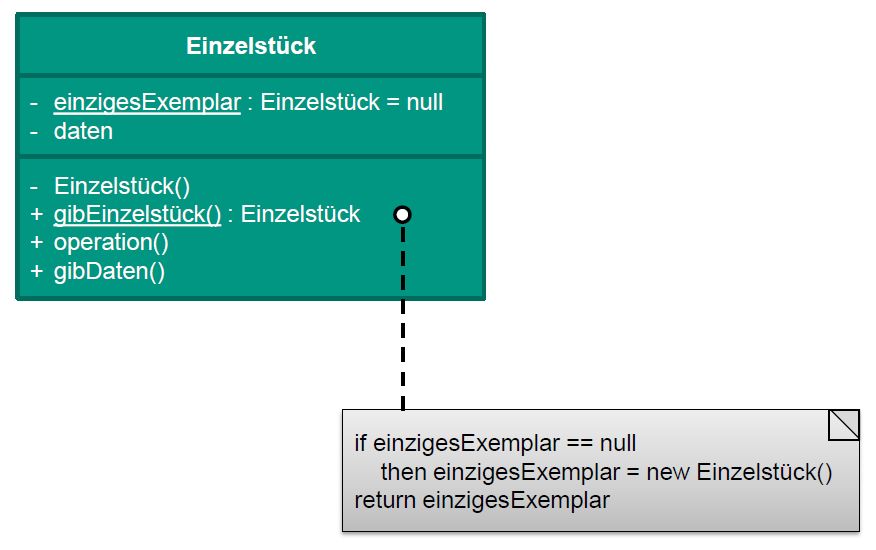
\includegraphics[width=0.7\textwidth]{../images/einzelstueck.png}
\end{center}
\newpage
\item \textbf{Fliegengewicht}
\begin{itemize}
\item Nutzt Objekte \textbf{kleinster Granularität gemeinsam}, um große Mengen von ihnen \textbf{effizient zu speichern}
\end{itemize}
\begin{center}
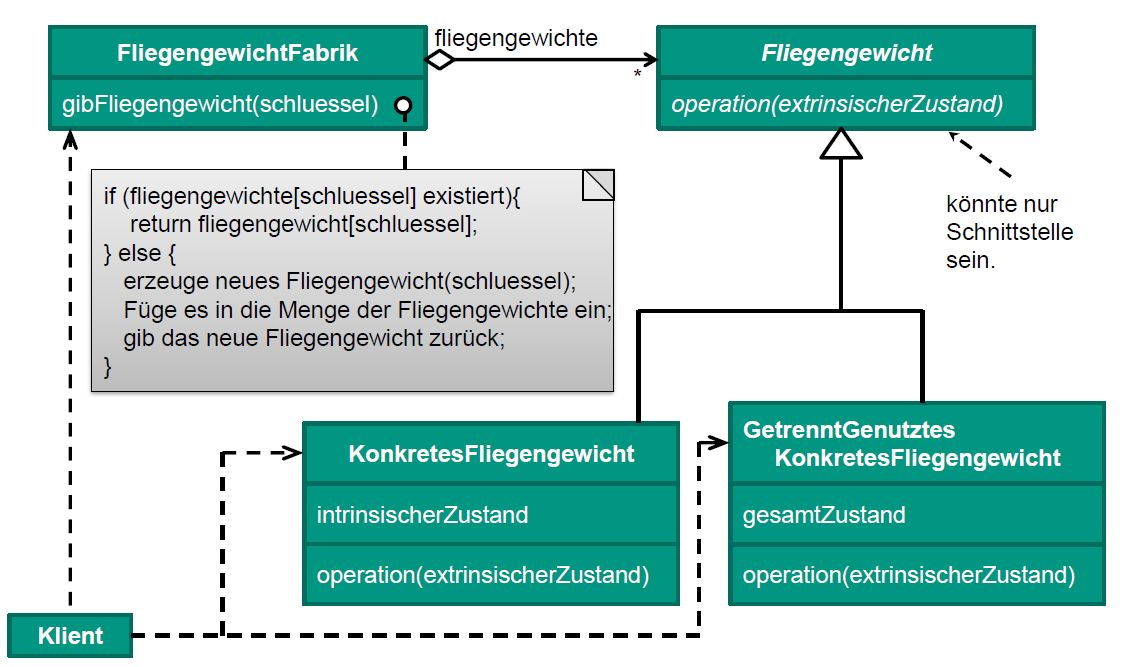
\includegraphics[width=0.8\textwidth]{../images/fliegengewicht.png}
\end{center}
\item \textbf{Memento}
\begin{itemize}
\item Erfasst und \textbf{externalisiert den internen Zustand eines Objekts}, ohne seine Kapselung zu verletzten, so dass das Objekt \textbf{später in diesen Zustand zurückversetzt} werden kann
\end{itemize}
\begin{center}
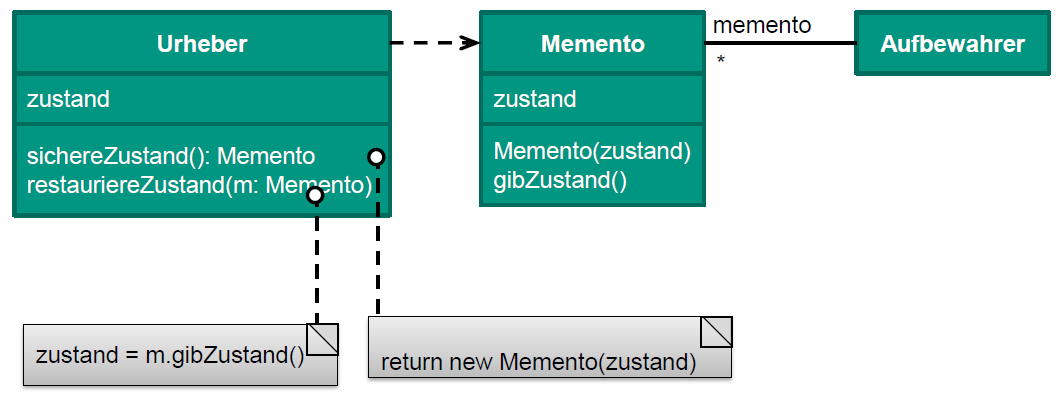
\includegraphics[width=0.9\textwidth]{../images/memento.png}
\end{center}
\newpage
\item \textbf{Prototyp}
\begin{itemize}
\item Bestimmt die \textbf{Arten zu erzeugender Objekte} durch die Verwendung eines typischen Exemplars und erzeuge neue Objekte durch \textbf{Kopieren dieses Prototyps}
\end{itemize}
\begin{center}
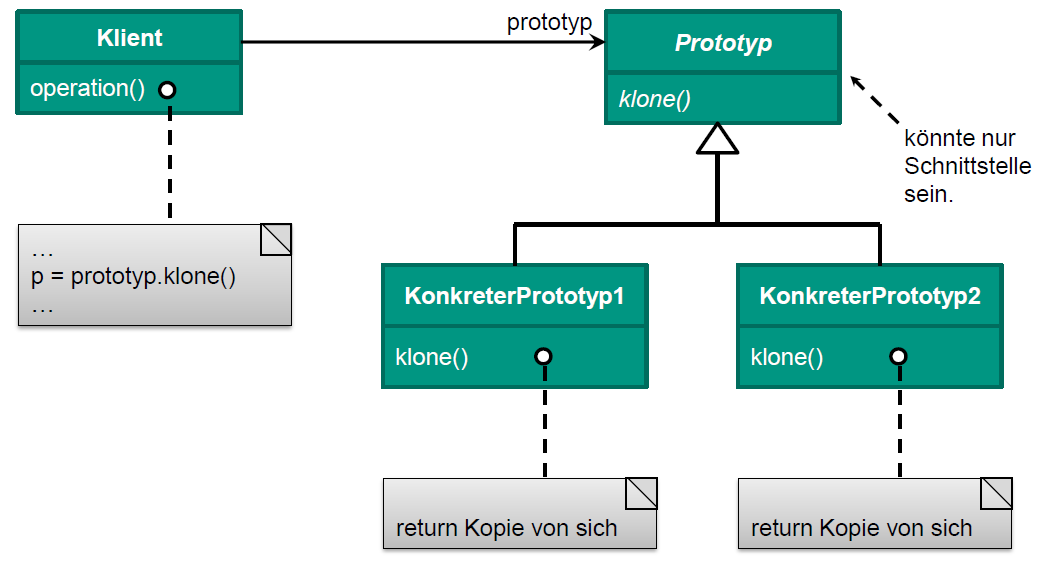
\includegraphics[width=0.9\textwidth]{../images/prototyp.png}
\end{center}
\item \textbf{Zustand}
\begin{itemize}
\item Ändere das \textbf{Verhalten} des Objekts, wenn sich dessen \textbf{interner Zustand ändert}
\end{itemize}
\begin{center}
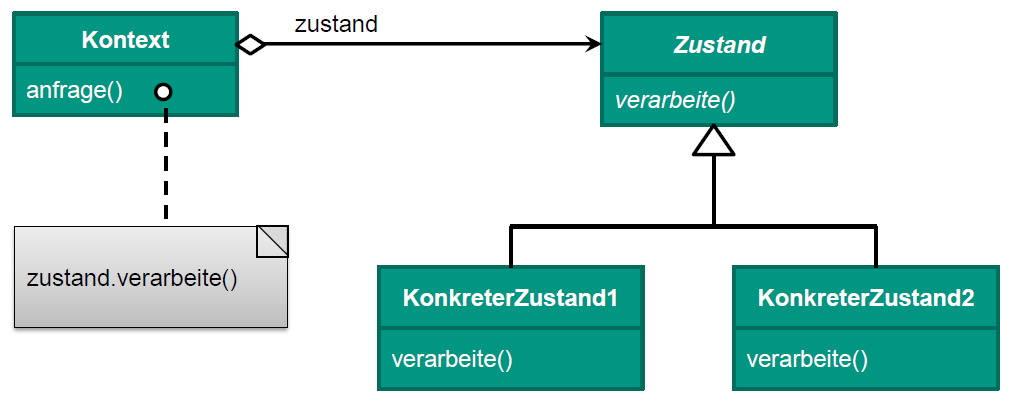
\includegraphics[width=0.9\textwidth]{../images/zustand.png}
\end{center}
\end{itemize}
			
\subsubsection{Steuerungsmuster}
			
\begin{itemize}
\item \textbf{Befehl}
\begin{itemize}
\item Kapselt einen \textbf{Befehl als Objekt} und ermöglicht es, Klienten mit verschiedenen \textbf{Anfragen zu parametrisieren}, Operationen in eine \textbf{Warteschlange} zu stellen, ein Logbuch zu führen und \textbf{Operationen rückgängig} zu machen
\end{itemize}
\begin{center}
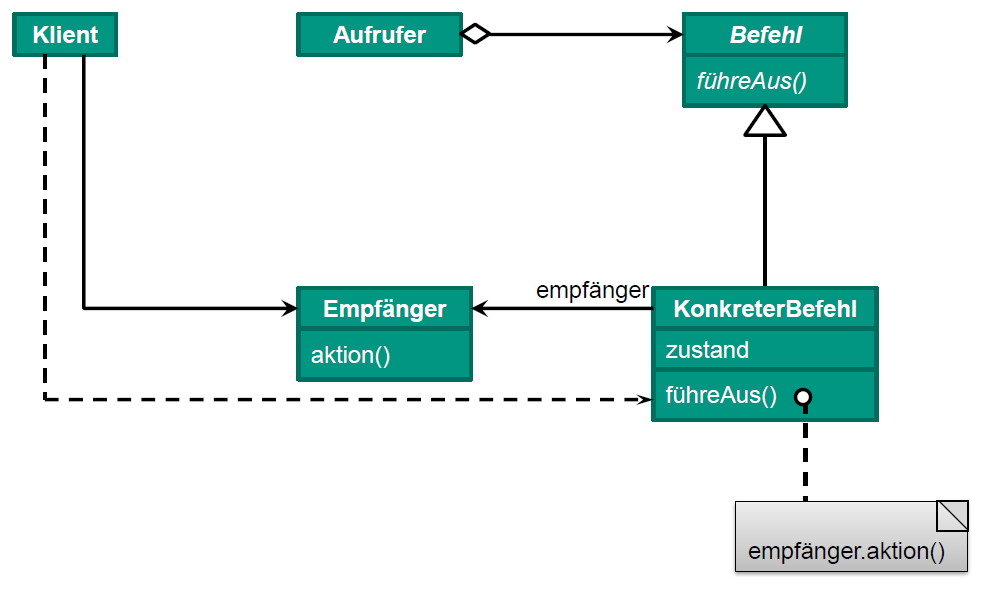
\includegraphics[width=0.7\textwidth]{../images/befehl.png}
\end{center}
\item \textbf{Master/Worker}
\begin{itemize}
\item Bietet \textbf{fehlertolerante- und parallele Berechnung}. Ein \textbf{Master verteilt die Arbeit an identische Worker} und \textbf{berechnet das Endergebnis} aus den Teilergebnissen, die die Worker zurückliefern
\end{itemize}
\begin{center}
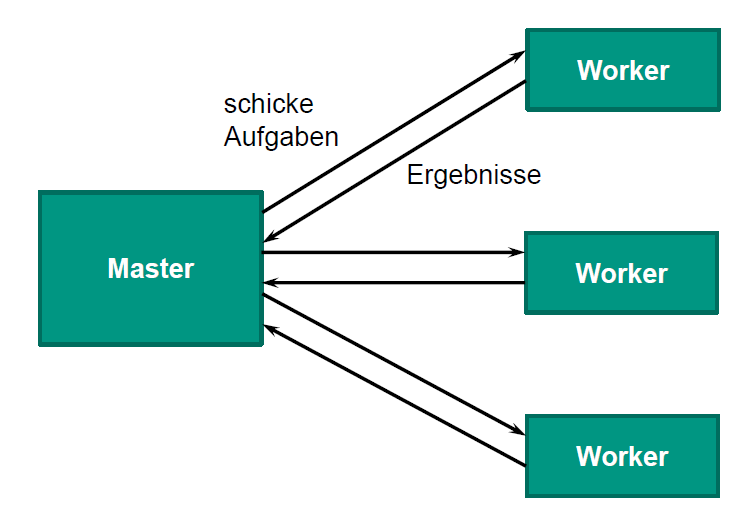
\includegraphics[width=0.6\textwidth]{../images/masterWorker.png}
\end{center}
\end{itemize}
	
\subsubsection{Bequemlichkeitsmuster}
		
\begin{itemize}
\item \textbf{Bequemlichkeitsklasse}
\begin{itemize}
\item \textbf{Vereinfachung von Methodenaufrufen} durch Bereithaltung der Parameter in \textbf{spezieller Klasse}
\end{itemize}
\begin{center}
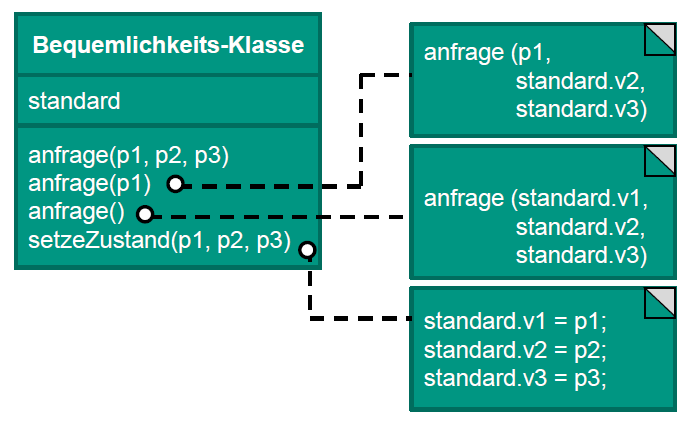
\includegraphics[width=0.8\textwidth]{../images/bequemlichkeitsklasse.png}
\end{center}
\item \textbf{Bequemlichkeitsmethode}
\begin{itemize}
\item \textbf{Vereinfachung von Methodenaufrufen} durch Bereithaltung \textbf{häufig genutzter Parameterkombinationen} in \textbf{zusätzlichen Methoden}
\end{itemize}
\begin{center}
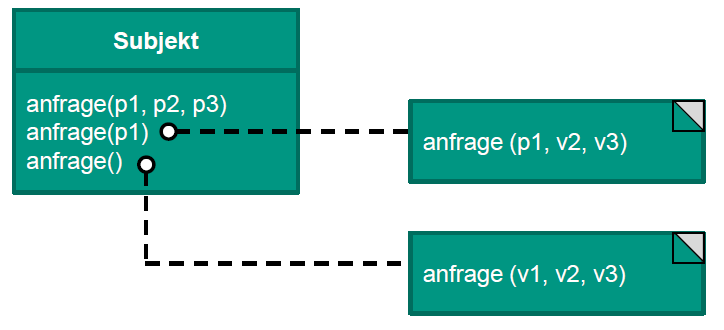
\includegraphics[width=0.8\textwidth]{../images/bequemlichkeitsmethode.png}
\end{center}
\newpage
\item \textbf{Fassade}
\begin{itemize}
\item Bietet \textbf{einheitliche Schnittstelle} zu einer \textbf{Menge von Schnittstellen} eines Subsystems
\begin{itemize}
\item Fassadenklasse bietet \textbf{abstrakte Schnittstelle}, die die Benutzung des Systems vereinfacht
\end{itemize}
\end{itemize}
\begin{center}
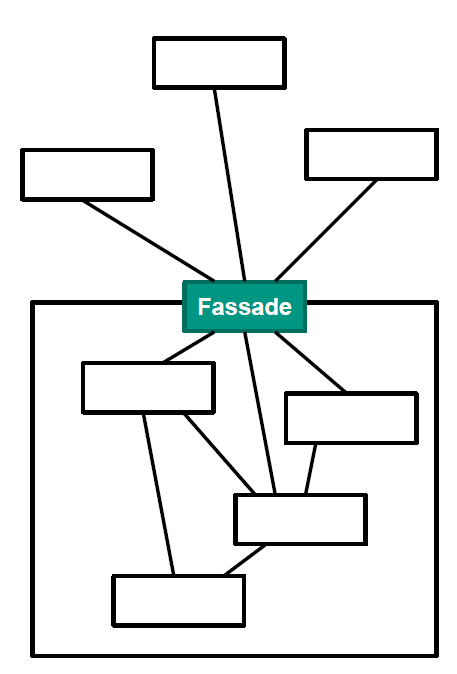
\includegraphics[width=0.3\textwidth]{../images/fassadeSchichtenarchitektur.png}
\end{center}
\item \textbf{Null-Objekt}
\begin{itemize}
\item Stellt \textbf{Stellvertreter} zur Verfügung, der die gleiche Schnittstelle bietet, aber \textbf{nichts tut}
\end{itemize}
\begin{center}
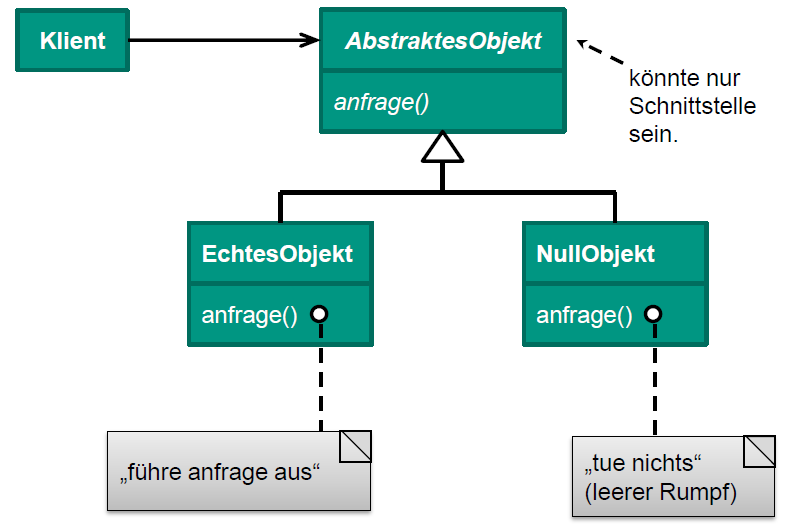
\includegraphics[width=0.6\textwidth]{../images/nullObjekt.png}
\end{center}
\end{itemize}
\addtocontents{toc}{\protect\newpage} % Seitenumbruch im Inhaltsverzeichnis
\newpage	
\section{Implementierungsphase}
	
Ziel:
				
\begin{itemize}
\item Leistungssteigerung durch \textbf{Parallelität}
\end{itemize}

\subsection{Grundlagen der Parallelität}
	
\begin{itemize}
\item Architekturstile:
\begin{itemize}
\item \textbf{Gemeinsamer Speicher} (Shared memory)
\begin{itemize}
\item CPUs haben \underline{einen} Speicher
\end{itemize}
\item Verteilter Speicher
\begin{itemize}
\item CPU hat eigenen Speicher
\end{itemize}
\end{itemize}
\end{itemize}
		
\begin{center}
\begin{tabular}{c|c}
Prozess & Kontrollfaden (Thread) \\
\hline
- Aufgabe eines Programms & - Leichtgewichtige Aufgabe eines Prozesses \\
$\Rightarrow$ \textbf{Durch Betriebssystem erzeugt} & - Greift auf \textbf{Daten des Prozess} zu \\
\end{tabular}
\end{center}
	
\subsection{Parallelität in Java}
		
\subsubsection{Erzeugen von Kontrollfäden}
			
\begin{itemize}
\item Mit Hilfe von:
\begin{itemize}
\item Interface \textbf{Runnable}
\item Klasse \textbf{Thread}
\end{itemize}
\newpage
\item Skizzierter Ablauf:			
\end{itemize}
			
\begin{center}
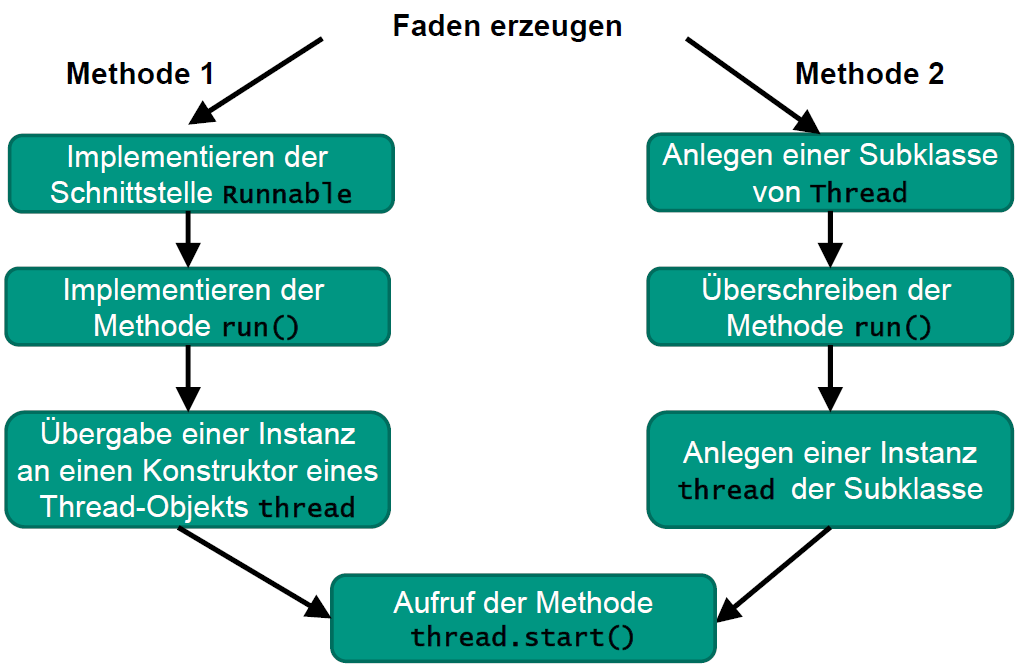
\includegraphics[width=0.7\textwidth]{../images/ablaufParallelitaetJava.png}
\end{center}
			
\begin{itemize}
\item Runnable vs. Thread:
\begin{itemize}
\item \textbf{Bessere Modularisierung} mit Runnable
\begin{itemize}
\item \textbf{Weniger Overhead} durch Kapselung
\item Aufgabe kann \textbf{über Netzwerk versendet} werden (\textbf{serialisierbar})
\end{itemize}
\end{itemize}
\end{itemize}
	
\subsubsection{Konstrukte zum Schützen kritischer Abschnitte}
	
\begin{itemize}
\item Koordination von:
\begin{itemize}
\item \textbf{Wechselseitigem Ausschluss}
\begin{itemize}
\item Eine Aktivität gleichzeitig!
\end{itemize}
\item \textbf{Warten auf Ereignisse/Benachrichtigungen}
\item \textbf{Unterbrechungen}
\begin{itemize}
\item Aktivität wartet auf ein (nicht) eintretendes Ereignis
\end{itemize}
\end{itemize}
\newpage
\item \underline{Wechselseitiger Ausschluss}
\begin{itemize}
\item Bei \textbf{gleichzeitigem Datenzugriff} kann es zu \textbf{Wettlaufsituationen} (race conditions) kommen:
\begin{itemize}
\item \textbf{Monitor} besetzt Aktivität bis zum Ende mit:
\begin{itemize}
\item \textbf{enter()}
\item \textbf{exit()}
\end{itemize}
\item Synchronisierung nach gleichem Prinzip mit:
\begin{itemize}
\item \textbf{synchronized (obj)}
\item \textbf{synchronized void foo()}
\end{itemize}
\end{itemize}
\item Monitor:
\end{itemize}
				
\begin{center}
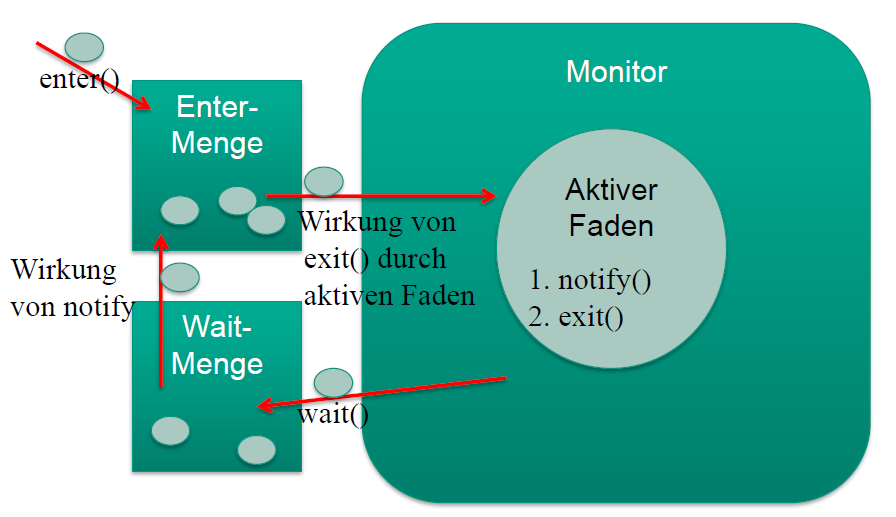
\includegraphics[width=0.8\textwidth]{../images/monitor.png}
\end{center}
				
\item \underline{Warten auf Ereignisse/Benachrichtigungen}
\begin{itemize}
\item Überprüfung, dass nur eine Aktivität gleichzeitig läuft, reicht nicht!
$\Rightarrow$ \textbf{Warteschlange} spielt eine Rolle!
\newpage
\item \underline{Methoden:}
\begin{itemize}
\item wait(), notify(), notifyAll() nur im \textbf{synchronized-Block}!

$\Rightarrow$ Monitor ist \dq this\dq und \underline{kann weggelassen} werden
\newline
$\Rightarrow$ Falls \underline{nicht} im synchronized-Block: \textbf{IllegalMonitorStateException}
\end{itemize}
\item wait():
\begin{itemize}
\item Setzt Faden in \textbf{Wartezustand bis Signal} eintritt
					
\color{red}{$\Rightarrow$ IMMER in einer Schleife!}
\newline							
\color{red}{$\Rightarrow$ Bedingung VOR und NACH dem Warten prüfen!}
\end{itemize}
\item notify(), notifyAll():
\begin{itemize}
\item Schicken \textbf{Signale an wartende Aktivitäten}
							
\color{red}{$\Rightarrow$ Sicher ist nur: notifyAll()}
\end{itemize}
\end{itemize}
\item \underline{Unterbrechnungen}
\begin{itemize}
\item Wie \underline{beendet} man Aktivitäten, die auf \underline{nicht mehr eintreffende} Signale warten?
$\Rightarrow$ Durch \textbf{interrupt()}
\item Die Methode \textbf{wait()} kann auch eine \textbf{InterruptedException} werfen!
\end{itemize}
\item \underline{Verklemmungen (Deadlocks)}
\begin{itemize}
\item \textbf{Semaphore}, die mit \underline{Anzahl an Genehmigungen} initialisiert werden
\begin{itemize}
\item \textbf{acquire():} Blockiert bis Genehmigung verfügbar und dann Genehmigungen--
\item \textbf{release():} Genehmigungen++
\end{itemize}
\item \textbf{CyclicBarrier}, die \underline{Gruppen von Fäden} synchronisiert
\begin{itemize}
\item Fäden rufen \textbf{await()} auf, die so lange blockiert, \underline{bis alle Fäden warten}
\end{itemize}
\end{itemize}
\end{itemize}
		
\newpage
\subsubsection{Bewertung von parallelen Algorithmen}
			
\begin{itemize}
\item \textbf{Beschleunigung:}
\begin{itemize}
\item {\LARGE ${S}{\left(p\right)}=\frac{T\left(1\right)}{T\left(p\right)}$}
\item ${S}{\left(p\right)}$ = Angabe, wie viel schneller mit p Prozessoren
\end{itemize}
\item \textbf{Effizienz:}
\begin{itemize}
\item {\LARGE ${E}{\left(p\right)}=\frac{T\left(1\right)}{p\cdot T\left(p\right)}=\frac{{S}{\left(p\right)}}{p}$}
\item ${E}{\left(p\right)}$ = Anteil an Ausführungszeit der nützlich verrichteten Arbeit
\begin{itemize}
\item \underline{Ideal:} ${S}{\left(p\right)} = {p}$ oder ${E}{\left(p\right)} = {1}$
\end{itemize}
\end{itemize}
\item \textbf{Gesamtlaufzeit:}
\begin{itemize}
\item {\LARGE ${T}{\left(p\right)} = \sigma + \frac{\pi}{{p}}$}
\item $\sigma$ = Zeit für Ausführung des sequentiellen Teils
\item $\pi$ = Zeit für die sequentielle Ausführung des parallelen Teils
\item ${p}$ = Anzahl an CPUs
\end{itemize}
\item \textbf{Amdahl'sches Gesetz:}
\begin{itemize}
\item {\LARGE ${S}{\left(p\right)} \le \frac{1}{f}$} mit {\LARGE ${f} = \frac{\sigma}{\sigma + \pi}$}
\end{itemize}
\end{itemize}
\newpage
\section{Testphase}
	
	Ziel:		
	\begin{itemize}
		\item Softwarefehler möglichst \textbf{früh finden}
		\begin{itemize}
			\item \textbf{Zeit ist Geld!}
		\end{itemize}
	\end{itemize}
		
	\subsection{Fehlerarten}
		
		\begin{itemize}
			\item \textbf{Irrtum/Herstellungsfehler:} Menschliche Aktion, die zum Defekt führt
			\item \textbf{Defekt:} Mangel an Softwareprodukt
			\item \textbf{Versagen/Ausfall:} Abweichung des Softwareverhaltens
		\end{itemize}
			
	\subsection{Fehlerklassen}
	
		\begin{itemize}
			\item \textbf{Anforderungsfehler} (Defekt im Pflichtenheft)
			\begin{itemize}
				\item Inkorrekte Benutzerwünsche,..
			\end{itemize}
			\item \textbf{Entwurfsfehler} (Defekt in der Spezifikation)
			\begin{itemize}
				\item Unvollständige/fehlerhafte Umsetzung der Anforderung,..
			\end{itemize}
			\item \textbf{Implementierungsfehler} (Defekt im Programm)
			\begin{itemize}
				\item Fehlerhafte Umsetzung der Spezifikation im Programm,..
			\end{itemize}
		\end{itemize}
		
	\subsection{Arten von Testhelfern}
			
		\begin{itemize}
			\item \textbf{Stummel}: Rudimentär implementierter Softwareteil
			\item \textbf{Attrappe}: Simuliert die Implementierung zu Testzwecken
			\item \textbf{Nachahmung}: Attrappe mit zusätzlicher Funktion
		\end{itemize}
	
	\subsection{Testphasen}
			
		\begin{center}
			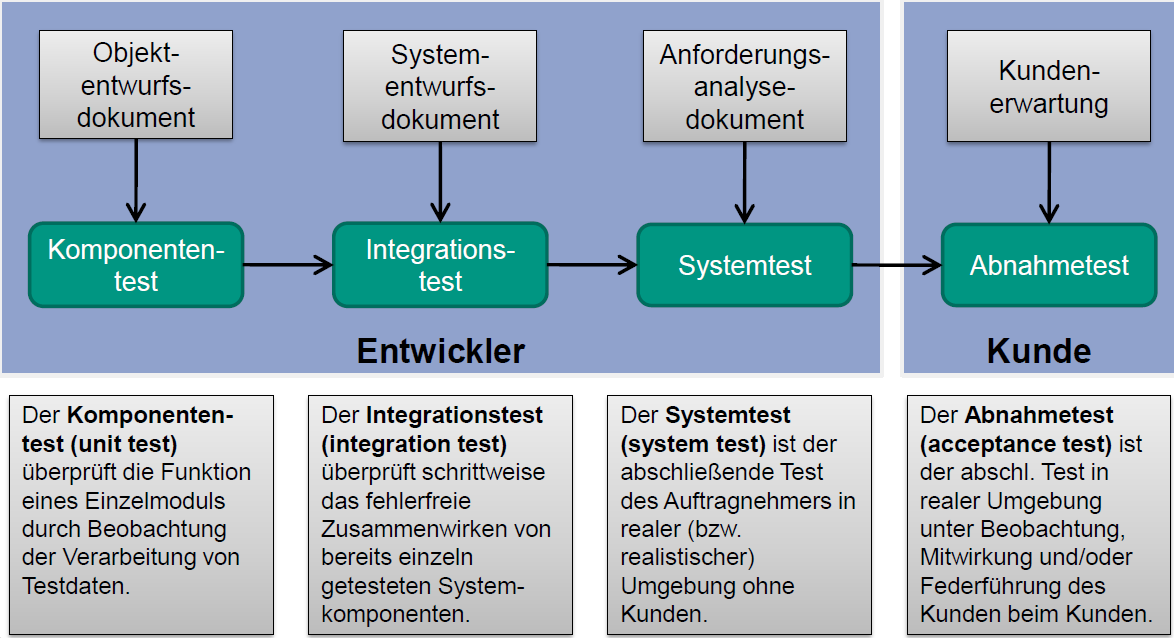
\includegraphics[width=0.8\textwidth]{../images/testphasen.png}
		\end{center}
		
	\subsection{Klassifikation testender Verfahren}
			
		\begin{itemize}
			\item \textbf{Dynamische Verfahren}
			\begin{itemize}
				\item Strukturtests
				\begin{itemize}
					\item Kontroll- und datenflussorientierte Tests
				\end{itemize}
				\item Funktionale Tests
				\item Leistungstests
			\end{itemize}
			\item \textbf{Statische Verfahren}
			\begin{itemize}
				\item Manuelle Prüfmethoden
				\item Prüfprogramme
			\end{itemize}
		\end{itemize}
			
		\newpage
		\subsubsection{Kontrollflussorientierte Testverfahren}
					
			\begin{itemize}
				\item \textbf{Anweisungsüberdeckung}
				\begin{itemize}
					\item Ausführung aller \textbf{Grundblöcke}
				\end{itemize}
				\item \textbf{Zweigüberdeckung}
				\begin{itemize}
					\item \textbf{Traversierung} aller Zweige
				\end{itemize}
				\item \textbf{Pfadüberdeckung}
				\begin{itemize}
					\item Ausführung aller \textbf{unterschiedlichen, vollständigen Pfade} im Programm
					\begin{itemize}
						\item Pfadanzahl \textbf{wächst bei Schleifen} enorm!
												
						$\Rightarrow$ \textbf{Nicht praktikabel!}
					\end{itemize}
				\end{itemize}
				\item Beispiel:
				\begin{center}
					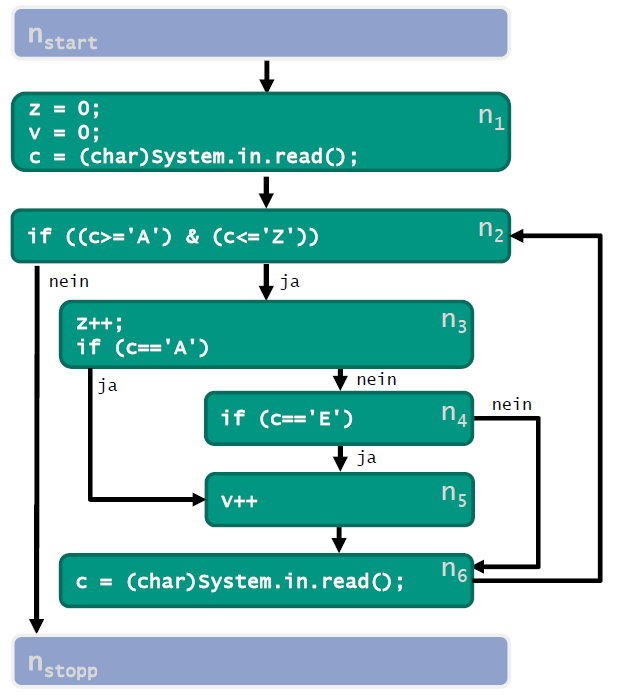
\includegraphics[width=0.6\textwidth]{../images/kfg.png}
				\end{center}
			\end{itemize}
	
		\subsubsection{Funktionale Tests}
			
			\begin{itemize}
				\item \textbf{Funktionale Äquivalenzklassenbildung}
				\begin{itemize}
					\item \textbf{Zerlege Wertebereich} der Eingabeparameter und \textbf{Definitionsbereich} der Ausgabeparameter in Äquivalenzklassen
				\end{itemize}
				\item \textbf{Grenzwertanalyse}
				\begin{itemize}
					\item Erweiterung von Äquivalenzklassenbildung mit \textbf{Grenzwerten}
				\end{itemize}
				\item \textbf{Zufallstest}
				\begin{itemize}
					\item \textbf{Zufällige Testfälle} (mit Testhelfern)
				\end{itemize}
				\item \textbf{Test von Zustandsautomaten}
				\begin{itemize}
					\item Testfälle aus \textbf{Zustandsübergängen}
				\end{itemize}
			\end{itemize}
		
		\subsubsection{Leistungstests}
				
			\begin{itemize}
				\item \textbf{Lasttests}
				\begin{itemize}
					\item Zuverlässigkeit und Einhalten der Spezifikation \textbf{im erlaubten Grenzbereich}
				\end{itemize}
				\item \textbf{Stresstests}
				\begin{itemize}
					\item Verhalten des System \textbf{beim Überschreiten} der definierten Grenzen
				\end{itemize}
			\end{itemize}
		
		\subsubsection{Manuelle Prüfung}
			
			\begin{itemize}
				\item \textbf{Semantik} wird geprüft
				\item \textbf{Aufwendig} (20\% der Erstellungskosten)
			\end{itemize}
	
		\subsubsection{Prüfprogramme}
				
			\begin{itemize}
				\item Warnungen, Fehler, Programmierstil, etc.
			\end{itemize}
	
		\subsubsection{Integrationstests}
			
			\begin{center}
				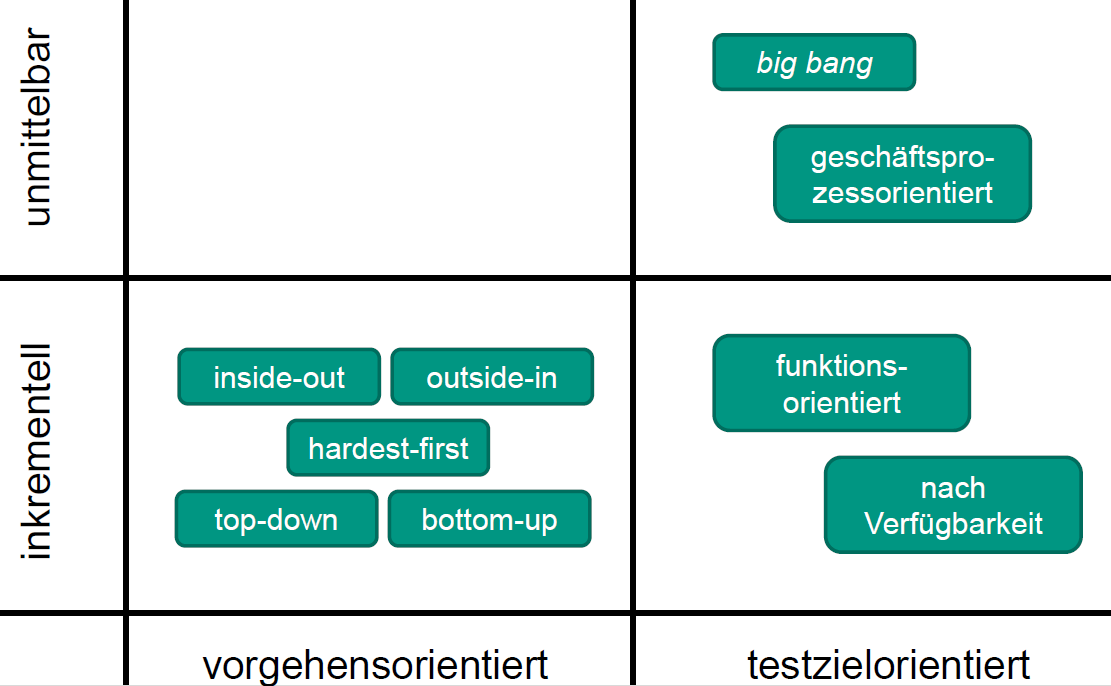
\includegraphics[width=0.6\textwidth]{../images/integrationstests.png}
			\end{center}
		
		\subsubsection{Systemtests}
				
			\begin{itemize}
				\item \textbf{Funktionaler Systemtest}
				\begin{itemize}
					\item Überprüfung funktionaler Qualitätsmerkmale, Korrektheit und Vollständigkeit
				\end{itemize}
				\item \textbf{Nichtfunktionaler Systemtest}
				\begin{itemize}
					\item Überprüfung nichtfunktionaler Qualitätsmerkmale wie: Sicherheit, Benutzbarkeit,..
				\end{itemize}
			\end{itemize}
		
		\subsubsection{Abnahmetests}
					
			\begin{itemize}
				\item Spezieller Systemtest: \textbf{Kunde beobachtet} oder \textbf{wirkt mit!}
				\item Formale Abnahme ist \textbf{bindende Erklärung der Annahme} durch den Auftraggeber
			\end{itemize}
		
	\subsection{Inspektion}
			
		\begin{itemize}
			\item \textbf{Phasen:}
			\begin{itemize}
				\item \textbf{Vorbereitung}
				\begin{itemize}
					\item \textbf{Teilnehmer/Rollen} festlegen
					\item \textbf{Dokumente/Formulare} vorbereiten
					\item \textbf{Zeitlichen Ablauf} planen
				\end{itemize}
				\item \textbf{Individuelle Fehlersuche}
				\begin{itemize}
					\item \textbf{Inspektoren prüfen} Dokumente für sich
					\item \textbf{Notieren der Problempunkte} und genaue Stelle im Dokument
					\item Problempunkte: Mögliche Defekte, Verbesserungsvorschläge, Fragen
				\end{itemize}
				\item \textbf{Gruppensitzung}
				\begin{itemize}
					\item \textbf{Problempunkte sammeln} und besprechen
					\item \textbf{Verbesserungsvorschläge sammeln}
				\end{itemize}
				\item \textbf{Nachbereitung}
				\begin{itemize}
					\item Liste der Problempunkte an \textbf{Editor}
					\item Editor identifiziert \textbf{tatsächliche Defekte} und \textbf{klassifiziert} sie
					\item \textbf{Alle Problempunkte} werden bearbeitet
				\end{itemize}
				\item \textbf{Prozessverarbeitung}
				\begin{itemize}
					\item \textbf{Standards für Dokumente} erarbeiten
					\item Defektklassifikationsschema, Planung und Durchführung verbessern
				\end{itemize}
			\end{itemize}
			\newpage
			\item \textbf{Rollen:}
			\begin{itemize}
				\item \textbf{Inspektionsleiter} (leitet alle Phasen)
				\item \textbf{Moderator} (leitet Gruppenphase)
				\item \textbf{Inspektor} (prüft Dokument)
				\item \textbf{Schriftführer} (protokolliert Defekte in Gruppensitzung)
				\item \textbf{Editor} (klassifiziert/behebt Defekte)
				\item \textbf{Autor} (verfasst Dokument)
			\end{itemize}
		\end{itemize}	
		\begin{center}
			\begin{tabular}{c|c}
				\color{green}{\textbf{+}}              & \color{red}{\textbf{-}} \\
				\hline
				- Anwendbar auf alle Softwaredokumente & - Aufwendig \\
				- Effektiv in industrieller Praxis     & - Teuer, da Zeitaufwand hoch \\
			\end{tabular}
		\end{center}
\newpage
\section{Abnahme-, Einführungs-, Wartungs- und Pflegephase}
	
	\subsection{Abnahmephase}
	
		\begin{itemize}
			\item \textbf{Übergabe des Gesamtprodukts} inklusive vollständiger Dokumentation
			\begin{itemize}
				\item Verbunden: \textbf{Abnahmeprotokoll und -test}
			\end{itemize}
		\end{itemize}
		
	\subsection{Einführungsphase}
	
		\begin{itemize}
			\item \textbf{Installation} des Produkts
			\item \textbf{Schulung} der Benutzer und des Benutzerpersonals
			\item \textbf{Inbetriebnahme} des Produkts:
			\begin{itemize}
				\item Direkte Umstellung
				\item Parallellauf
				\item Versuchslauf
			\end{itemize}
		\end{itemize}
			
	\subsection{Wartungs- und Pflegephase}
	
		\begin{itemize}
			\item Kategorien:
			\begin{itemize}
				\item Korrektive Tätigkeiten (\textbf{Wartung})
				\begin{itemize}
					\item Stabilisierung/Korrektur
					\item Optimierung/Leistungsverbesserung
				\end{itemize}
				\item Progressive Tätigkeiten (\textbf{Pflege})
				\begin{itemize}
					\item Anpassung/Änderung
					\item Erweiterung
				\end{itemize}
			\end{itemize}
		\end{itemize}
\newpage
\section{Aufwandsschätzung}
		
	\subsection{Schätzmethoden}
			
		\begin{itemize}
			\item \textbf{Analogiemethode}
			\begin{itemize}
				\item Vergleiche die zu schätzenden Entwicklungen mit \textbf{bereits abgeschlossenen Produktentwicklungen} anhand von \textbf{Ähnlichkeitskriterien}
			\end{itemize}
			\item \textbf{\textbf{Basismethoden}}
			\begin{itemize}
				\item \textbf{Relationsmethode}
				\begin{itemize}
					\item Methode, die anhand von \textbf{Faktoren} (Programmiersprache/-erfahrung, Dateiorganisation) vergleicht, wie diese den \textbf{Aufwand beeinflussen}: \textbf{Auf- und Abschläge} mit etwa gleich großem, existierenden Produkt
				\end{itemize}
				\item \textbf{Multiplikatormethode}
				\begin{itemize}
					\item \textbf{Zerlegung in Teilprodukte} mit Zuteilung feststehender Aufwände
									
					$\Rightarrow$ Anzahl Teilprodukte {\Large $\cdot$} Aufwand Kategorie
				\end{itemize}
				\item \textbf{Phasenaufteilung}
				\begin{itemize}
					\item Ermittlung aus abgeschlossenen Entwicklungen werden \textbf{auf einzelne Entwicklungsphasen verteilt} (Kuchendiagramm)
				\end{itemize}
			\end{itemize}
			\item \textbf{COCOMO II}
			\begin{itemize}
				\item {\LARGE $PM = A \cdot (Size)^{1,01 + 0,01 \cdot {\sum_{j=1}^{5} SF_{j}}} \cdot \prod_{i=1}^{17} EM_{i}$}
				\begin{itemize}
					\item $PM$ = Personenmonate
					\item $A$ = Konstante für Kalibrierung des Modells (z.B. LOC)
					\item $Size$ = Geschätzter Umfang der Software in KLOC
					\item $SF_{j}$ = Skalierungsfaktoren
					\item $EM_{i}$ = Multiplikative Kostenfaktoren
				\end{itemize}
			\end{itemize}
		\end{itemize}	
\newpage	
\section{Prozessmodelle}
	
\begin{itemize}
\item \textbf{Programmieren durch Probieren} (Trial \& Error)
\begin{itemize}
\item \textbf{Programm erzeugen und danach alles weitere} planen, testen, warten,..
				
\begin{center}
\begin{tabular}{c|c}
\color{green}{\textbf{+}} & \color{red}{\textbf{-}} \\
\hline
- Schnell & - Schlecht strukturiert \\
- Ohne nutzlosen Zusatzaufwand & - Keine Dokumentation
\end{tabular}
\end{center}
\end{itemize}
\item \textbf{Wasserfallmodell}
\begin{itemize}
\item \textbf{Dokumentgetriebenes Modell}
\item \textbf{Jede Aktivität in fester Reihenfolge} und anschließendem Dokument
				
\begin{center}
\begin{tabular}{c|c}
\color{green}{\textbf{+}} & \color{red}{\textbf{-}} \\
\hline
- Einfach & - Entwurf, Implementierung und Testen von nutzlosem Code \\
- Verständlich & - Keine Rückkopplung
\end{tabular}
\end{center}
\end{itemize}
\item \textbf{V-Modell 97} (Vorgehensmodell)
\begin{itemize}
\item Jede Aktivität hat \textbf{eigenen Prüfungsschritt}
\end{itemize}
\end{itemize}
		
\begin{center}
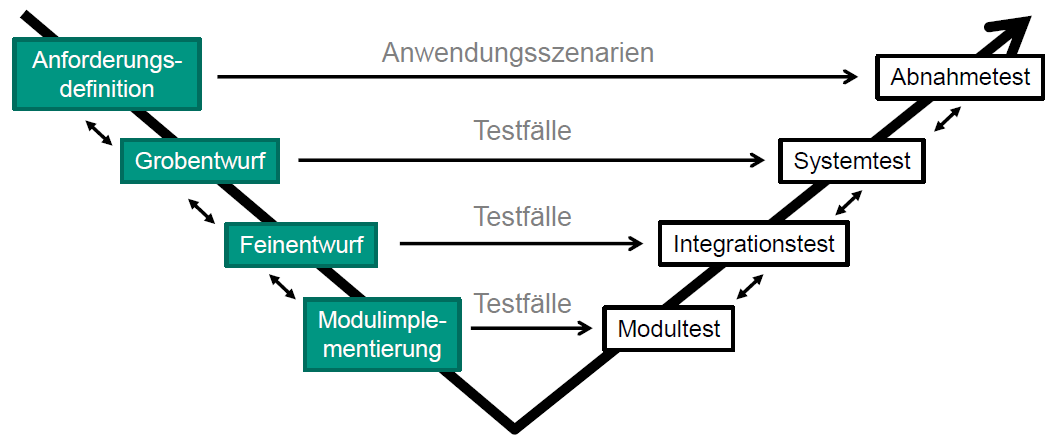
\includegraphics[width=0.9\textwidth]{../images/vmodell97.png}
\end{center}
				
\newpage
\begin{itemize}
\item \textbf{V-Modell XT}
\begin{itemize}
\item Entwicklungsstandard für IT-Systeme der \textbf{öffentlichen Hand}
\item \textbf{Aktivitäten, Produkte und Verantwortlichkeit} werden festgelegt, jedoch \underline{keine} Reihenfolge
\item Aufteilung in \textbf{vier Submodelle} mit zusätzlichen \textbf{Vorgehensbausteinen}:
\begin{itemize}
\item \textbf{Projektmanagement}
\item \textbf{Qualitätssicherung}
\item \textbf{Konfigurationsmanagement}
\item \textbf{Systemerstellung}
\end{itemize}
\end{itemize}
\item \textbf{Prototypmodell}
\begin{itemize}
\item Geeignet für Systeme, für die keine vollständige Spezifikation \textbf{ohne explorative Entwicklung/Experimentation} erstellt werden kann
\item Prototyp wird \textbf{WEGGEWORFEN!}
\end{itemize}
\item \textbf{Iteratives Modell}
\begin{itemize}
\item \textbf{Teile der Funktionalität} lassen sich \underline{klar} definieren/realisieren
\begin{itemize}
\item Funktionalität wird \textbf{Schritt für Schritt} hinzugefügt
\end{itemize}
\end{itemize}
\item \textbf{Synchronisiere und Stabilisiere}
\begin{itemize}
\item Idee:
\end{itemize}
			
\begin{center}
\begin{tabular}{c}
Programmierer in \textbf{kleinen Teams} \\
$\Downarrow$ \\
Regelmäßig \textbf{synchronisieren} (nächtlich) \\
$\Downarrow$ \\
Regelmäßig \textbf{stabilisieren} (3-Monate) \\
\end{tabular}
\end{center}
			
\newpage
\begin{itemize}			
\item \textbf{Phasen:}
\begin{itemize}
\item \textbf{Planungsphase} (3-12 Monate)
\begin{itemize}
\item Wunschbild, Spezifikation, Zeitplan und Teamstruktur
\end{itemize}
\item \textbf{Entwicklungsphase} (6-12 Monate)
\begin{itemize}
\item Manager koordinieren, Entwickler entwerfen und Tester testen parallel
\end{itemize}
\item \textbf{Stabilisierungsphase} (3-8 Monate)
\begin{itemize}
\item Manager koordinieren Beta-Tester und sammeln Rückmeldungen
\item Entwickler stabilisieren Code
\item Tester isolieren Fehler
\end{itemize}
\end{itemize}
\end{itemize}
\end{itemize}
					
\begin{center}
\resizebox{\textwidth}{!}{
\begin{tabular}{c|c}
\color{green}{\textbf{+}} & \color{red}{\textbf{-}} \\
\hline
- Effektiv durch kurze Produktzyklen & - Ungeeignet für manche Art von Softwareproblemen \\
- Fortschritt ohne vollständige Spezifikation & - Mangelnde Fehlertoleranz oder Echtzeitfähigkeit
\end{tabular}}
\end{center}
	
\subsection{Agile Prozessmodelle}
	
\begin{itemize}
\item Idee:
\begin{itemize}
\item \textbf{Minimum} an Vorausplanung
\item Planung erfolgt \textbf{inkrementell}
\item \textbf{Schnelle Reaktion} auf Änderung
\end{itemize}

\newpage
\item Vertreter:
\begin{itemize}
\item \textbf{Extreme Programming} (XP)
\item \textbf{Scrum!}
\item Crystal
\item Adaptive Software Development
\item Feature-Driven Development
\item Software Expedition
\end{itemize}
\end{itemize}
			
\subsubsection{Extreme Programming}
	
\begin{itemize}
\item \textbf{Paarprogrammierung}
\begin{itemize}
\item \underline{Zwei} Entwickler an \underline{einer} Maus/Tastatur
\item Geeignet für:
\begin{itemize}
\item \textbf{Vage und schnell ändernde} Anforderungen
\item \textbf{Kleines} Entwicklerteam
\item \textbf{Wenig} Verwaltungsaufwand
\end{itemize}
\end{itemize}
\end{itemize}
			
\begin{center}
\resizebox{\textwidth}{!}{
\begin{tabular}{c|c}
\color{green}{\textbf{+}} & \color{red}{\textbf{-}} \\
\hline
- Bessere Qualität des Quellcodes & - Doppelte Kosten \\
- Gut für unerfahrene Entwickler & - Vorteil gegenüber einzelner Programmierung \\ 
& mit Inspektionen nicht nachweisbar
\end{tabular}}
\end{center}
		
\newpage
\subsubsection{Scrum}
			
\begin{itemize}
\item Vorgehensmodell: \textbf{Agiles Projektmanagement}
\item \textbf{Artefakte:}
\begin{itemize}
\item \textbf{Anforderungsliste} (Product backlog)
\begin{itemize}
\item \underline{Produktanforderungen} und Liste aller \underline{Projektarbeiten}
\item Anforderungen vor jedem Sprint \underline{priorisiert}
\end{itemize}
\item \textbf{Aufgabenliste} (Sprint backlog)
\begin{itemize}
\item Alle Aufgaben mit Beschreibungen für \underline{aktuellen Sprint}
\end{itemize}
\item \textbf{Hindernisliste} (Impediment backlog)
\begin{itemize}
\item Alle \underline{Hindernisse des Projekts}, die Scrum-Master mit Team bespricht
\end{itemize}
\end{itemize}
\item \textbf{Rollen:}
\begin{itemize}
\item \textbf{Auftraggeber} (Product owner)
\begin{itemize}
\item Legt \underline{Anforderungen/Auslieferungstermin} fest
\item Stellt \underline{Budget}
\item \underline{Priorisiert} Anforderungen für Sprint
\end{itemize}
\item \textbf{Scrum-Master}
\begin{itemize}
\item Sicherstellung der \underline{Scrumwerte und -techniken}
\item Sorgt sich um \underline{vollständiges, funktionsfähiges und produktives Team}
\item \underline{Beseitigt Hindernisse} und kommuniziert zwischen den Rollen
\end{itemize}
\item \textbf{Entwicklungsteam}
\begin{itemize}
\item Personen \underline{unterschiedlicher Fachrichtungen}
\end{itemize}
\end{itemize}

\newpage
\item \textbf{Treffen:}
\begin{itemize}
\item \textbf{Sprintplanung}
\begin{itemize}
\item Entwicklungsteam wählt \underline{machbare Anforderungen} aus, die im Sprint geschafft werden kann und erstellt mit Scrum-Master eine Aufgabenliste
\end{itemize}
\item \textbf{Tägliches Scrumtreffen} (Daily Scrum)
\begin{itemize}
\item \dq Was hast du gestern getan?\dq
\item \dq Was wirst du heute tun?\dq
\item \dq Welche Hindernisse gibt es?\dq
\end{itemize}
\item \textbf{Reviewtreffen} (Sprintende)
\begin{itemize}
\item Vorstellen der \underline{Sprintergebnisse}
\item \underline{Keine} Folien!
\end{itemize}
\item \textbf{Retrospektive}
\begin{itemize}
\item \underline{Analyse vom letzten Sprint} mit dem Entwicklungsteam, Scrum-Master, Auftraggeber und eventuell dem Endkunden
\end{itemize}
\end{itemize}
\end{itemize}
\newpage
\section{Werkzeugkette und Versionskontrolle}
	
	\subsection{Befehlskette}
		
		git <Kommando>:
		
		\begin{itemize}
			\item \textbf{help:} Liste der Kommandos
			\item \textbf{init:} Depot anlegen
			\item \textbf{clone:} Depot eines Projekts laden
			\item \textbf{add:} Neue Datei hinzufügen und in Staging Area übernehmen
			\item \textbf{commit:} Änderungen in das eigene Depot übernehmen
			\item \textbf{push:} Commits in ein anderes Depot übertragen
			\item \textbf{fetch:} Änderungen von einem anderen Depot holen
			\item \textbf{merge:} Änderungen von einem Branch in einen anderen übertragen
			\item \textbf{pull:} Ausführen von fetch und merge
		\end{itemize}
		
	\subsection{Interaktion innerhalb Local- und Remote Repository}
		
		\begin{center}
			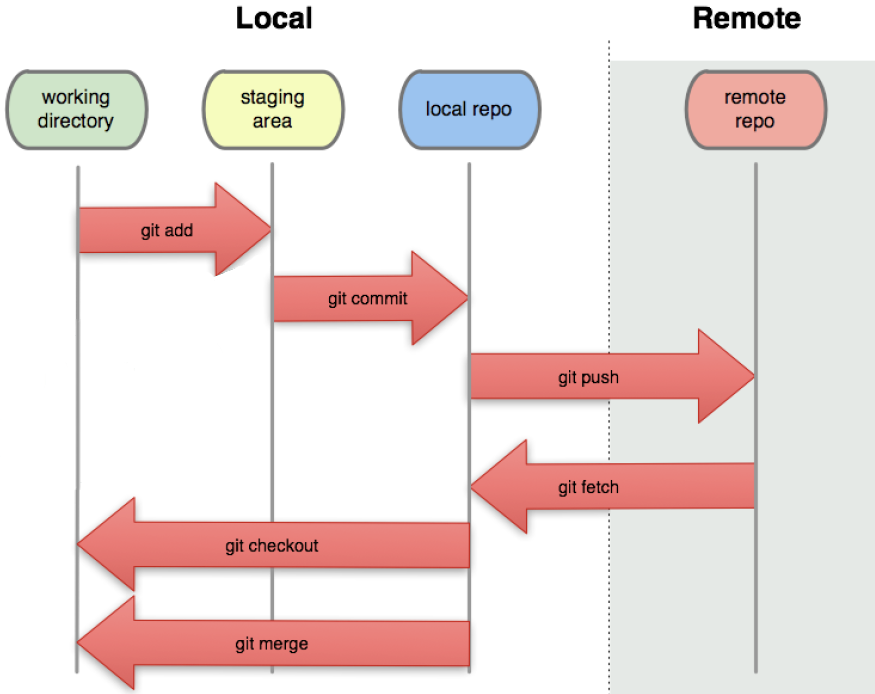
\includegraphics[width=0.57\textwidth]{../images/gitInteraktion.png}
		\end{center}
		
	\subsection{Unterschied: GIT und SVN}
		
		\begin{center}
			\begin{tabular}{c|c}
				\textbf{GIT}                                      & \textbf{SVN} \\
				\hline
				- Depot ist für jeden User \textbf{lokal}         & - Depot wird \textbf{auf einem Server} abgelegt \\
				- Operationen \textbf{offline ausführbar}         & - \textbf{Optimistisches Ausbuchen} \\
				- \textbf{Kryptografische Sicherung} der Historie & - Versioniert gesamtes Depot \\
				- Speichert \textbf{Schnappschüsse}               & - Speichert \textbf{Deltas} \\
			\end{tabular}
		\end{center}
		
	\subsection{Versionskontrolle}
		
		\subsubsection{Vorwärtsdelta}
		
			\textbf{Anfangsversion als Ausgangspunkt} und alle Deltas danach werden gespeichert.
			
		\subsubsection{Rückwärtsdelta}
			
			\textbf{Neueste Version als Ausgangspunkt} und alle Deltas davor werden gespeichert.
				
			\begin{tabular}{c|c|c}
				               & \textcolor{green}{\textbf{+}}      & \textcolor{red}{\textbf{-}} \\
				\hline
				Vorwärtsdelta  & Schneller Zugriff auf alte Version & Langsamer Zugriff auf alte Version \\
				\hline
				Rückwärtsdelta & Schneller Zugriff auf alte Version & Langsamer Zugriff auf neue Version \\
			\end{tabular}
			
		\subsubsection{Ein- und Ausbuchen}
		
			\begin{itemize}
				\item Optimistisch: \textbf{Mehrfaches} Ein- und Ausbuchen \textbf{ohne Änderungsreservierung}
				\item Strikt: Ein- und Ausbuchen \textbf{mit Änderungsreservierung}
			\end{itemize}		
\newpage
\section{Quellenverzeichnis}
	
\subsection{Literatur}
	
\begin{itemize}
\item Alle Informationen wurden den Vorlesungsfolien aus dem Kurs Softwaretechnik 1 vom Sommersemester 2018 des Karlsruher Instituts für Technologie entnommen.
\end{itemize}
	
\subsection{Grafiken}
		
\begin{itemize}
\item Alle Grafiken wurden den Vorlesungsfolien aus dem Kurs Softwaretechnik 1 vom Sommersemester 2018 des Karlsruher Instituts für Technologie entnommen.
\end{itemize}
	
\end{document}